\fakesection{Classification}{\hfill\small\texttt{/src/session\_1.m}, \texttt{/src/homework\_1.m}}

\begingroup
\setlength{\columnsep}{0.5cm}
\setlength{\intextsep}{0.5cm}
\begin{wrapfigure}{r}{0pt}
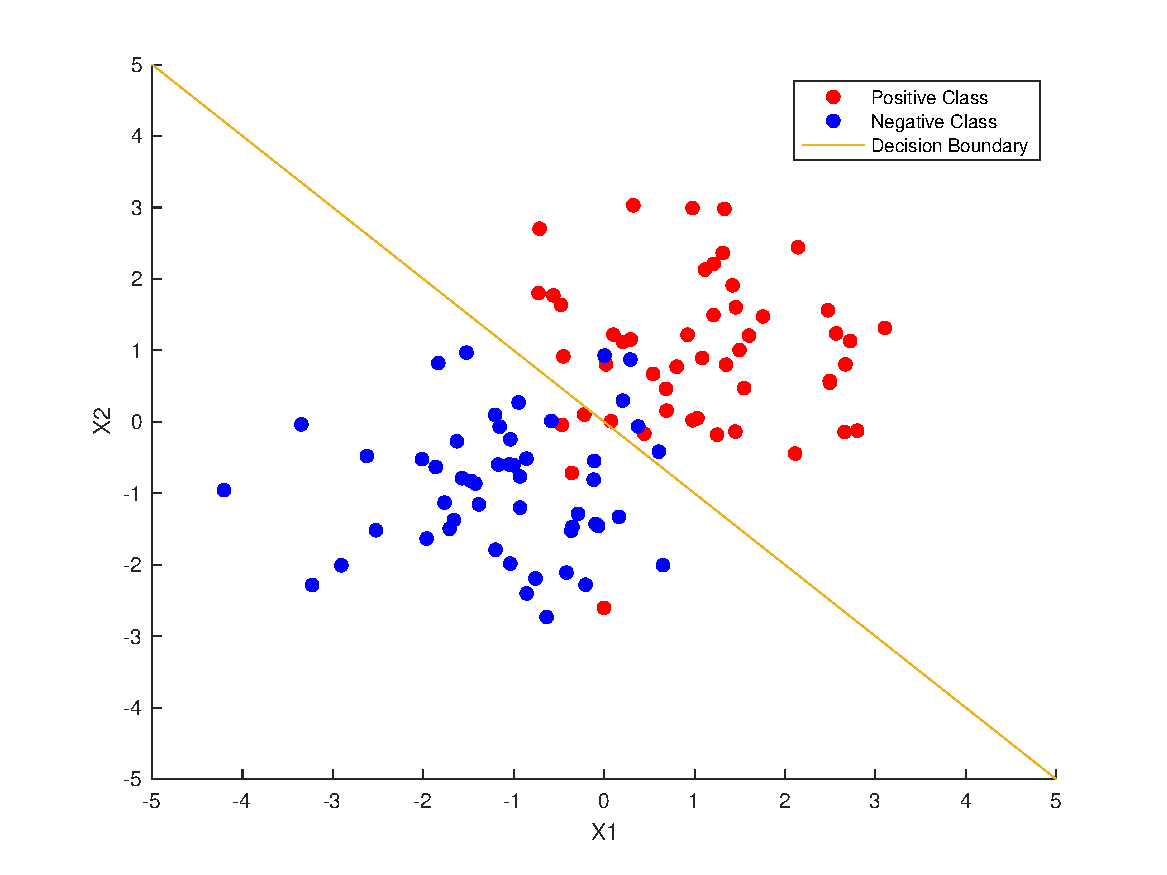
\includegraphics[width=0.45\textwidth]{../src/figures/twogaussians.pdf}
\caption{Decision boundary (in orange) for two Gaussian distributions with equal covariance matrices.}
\label{twogaussians}
\end{wrapfigure}
\fakesubsection{Two Gaussians}{}
For a binary classifier where the distributions are (assumed or known to be) Gaussian with equal covariance matrices the decision boundary that maximises the posterior probability $P(C_i|x)$ becomes linear. This is independent of the amount of overlap. Trying to get a better boundary would lead to overfitting. In this particular example where $\Sigma_{xx}=\mathbb{I}$ one ends up with a perpendicular bisector of the segment connecting the two cluster means 
$(-1,-1)$ and $(1,1)$, which gives $f(x)=-x$ as a decision boundary.
\fakesubsection{Support Vector Machine Classifier}{}
To deal with the non-linearly separable classification problem in the example one solves the following minimisation problem, where the hyperparameter $C$ controls the tradeoff between maximising the margin and making sure that the data lies on the correct side of that margin :

\endgroup
\vspace{-0.5cm}
$$\min_x\frac{1}{2}\cdot w^T\cdot w+C\cdot \sum_{k=1}^N\xi_k\qquad\text{such that $y_k\cdot[w^T\cdot x_k+b]\geq 1-\xi_k$ and $\xi_k\geq 0$ $(\forall k\in\{1,..,N\})$}$$
A dual form can be expressed by making use of Lagrange multipliers which in this context are also called \textit{support values}. Any data points for which the corresponding support value isn't zero are called \textit{support vectors}. These lie close to the boundary or are misclassified\footnote{In the dual problem formulation the $\alpha$ values are minimised for those data points that are `similar' to data points that belong to the same class.}.

\begin{figure}[ht]
\centering
\subfloat[$C = 0.01$ (large margin, lots of \textit{`slacking'}.)]{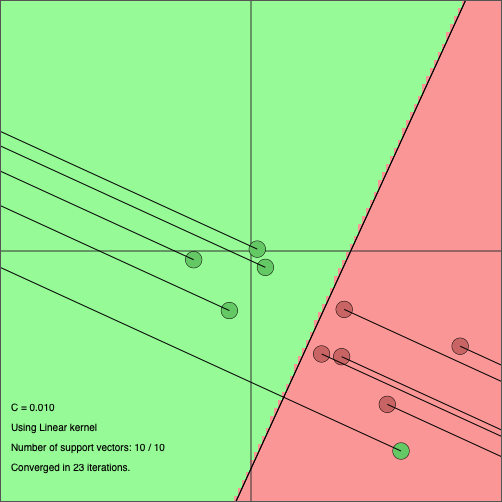
\includegraphics[width=0.17\textwidth]{../src/figures/stanford/canvas01}}\qquad
\subfloat[$C = 1$]{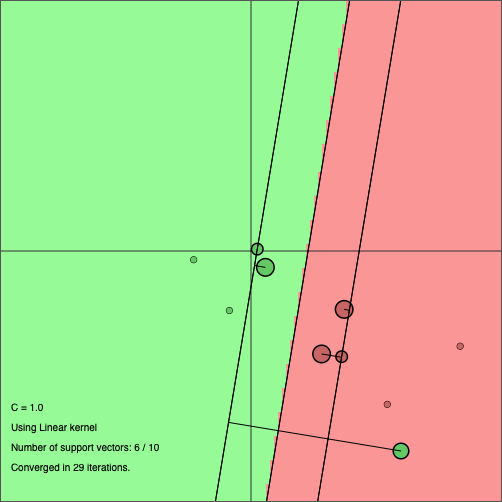
\includegraphics[width=0.17\textwidth]{../src/figures/stanford/canvas1}}\qquad
\subfloat[$C = 10$ (small margin, little \textit{`slacking'}.]{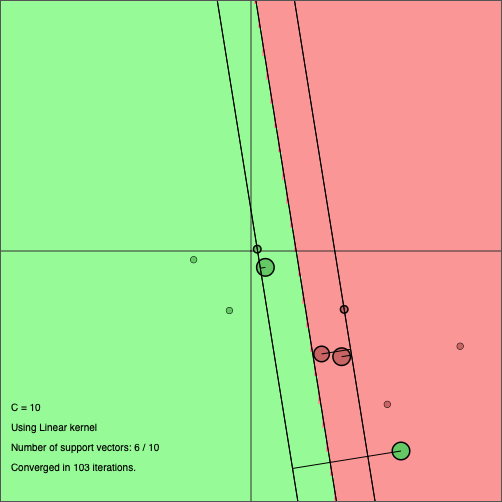
\includegraphics[width=0.17\textwidth]{../src/figures/stanford/canvas10}}\\
\subfloat[Initial solution.]{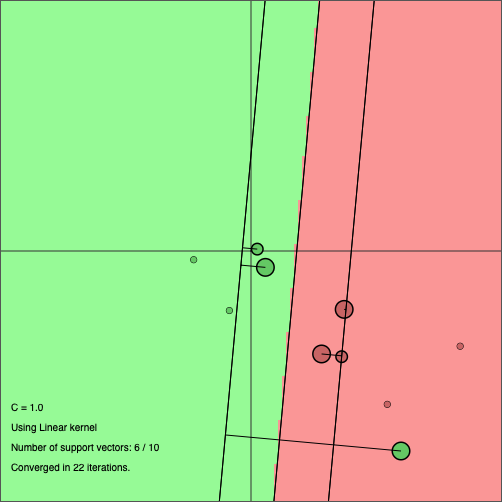
\includegraphics[width=0.17\textwidth]{../src/figures/stanford/canvasnew}}\qquad
\subfloat[Negative data points added at the right side of the margin.]{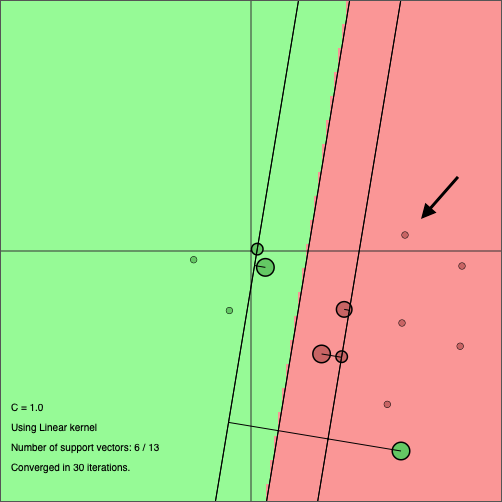
\includegraphics[width=0.17\textwidth]{../src/figures/stanford/canvasnew2}}\qquad
\subfloat[Negative data point added at the other side of the margin.]{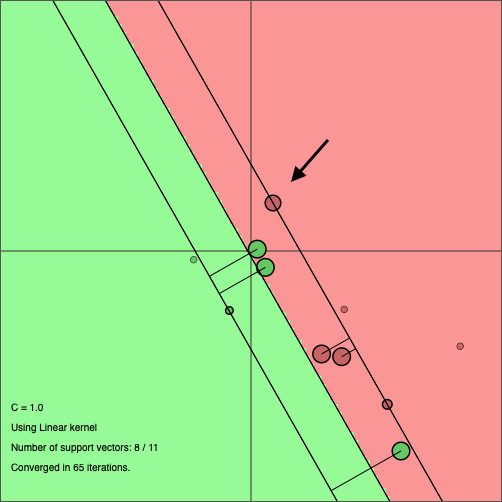
\includegraphics[width=0.17\textwidth]{../src/figures/stanford/canvasnew3}}\\
\subfloat[$\sigma=0.1$]{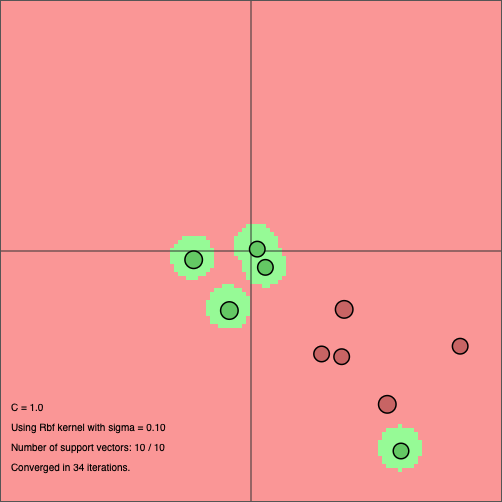
\includegraphics[width=0.17\textwidth]{../src/figures/stanford/canvasrbf025}}\qquad
\subfloat[$\sigma=1.0$]{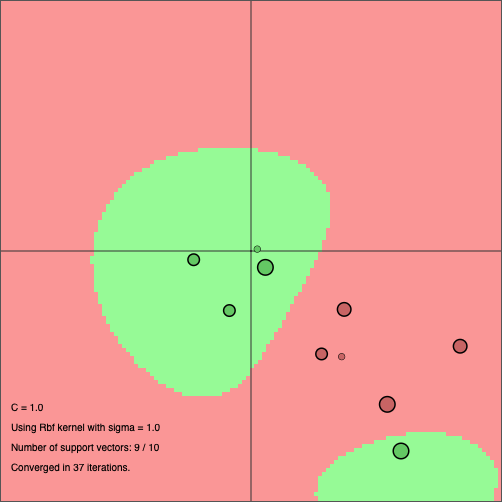
\includegraphics[width=0.17\textwidth]{../src/figures/stanford/canvasrbf1}}\qquad
\subfloat[$\sigma=100$]{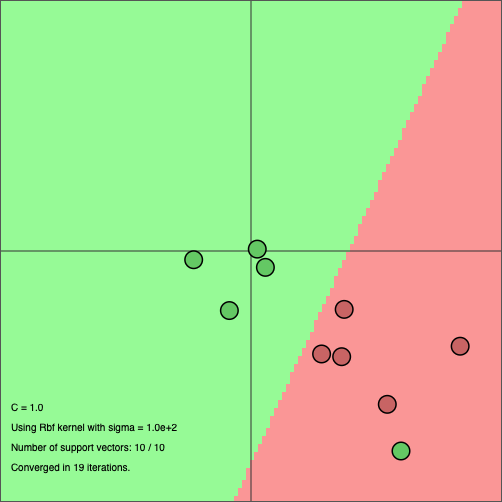
\includegraphics[width=0.17\textwidth]{../src/figures/stanford/canvasrbf100}}\\
\subfloat[Negative data point added far away from the boundary.]{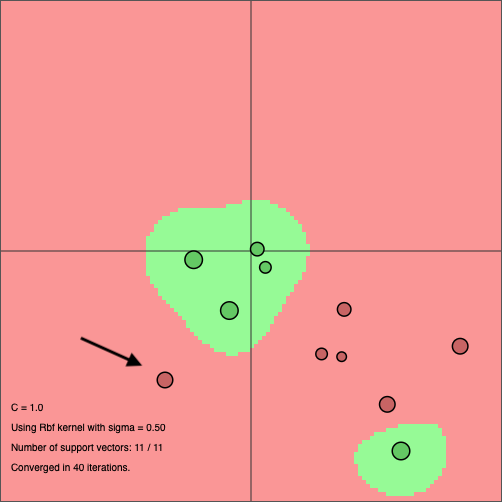
\includegraphics[width=0.17\textwidth]{../src/figures/stanford/canvasnewrbf1}}\qquad
\subfloat[Positive data point added inside the boundary.]{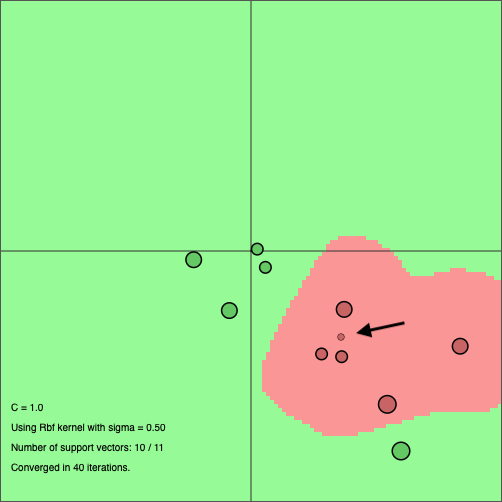
\includegraphics[width=0.17\textwidth]{../src/figures/stanford/canvasnewrbf2}}\qquad
\subfloat[Positive data point added inside the boundary.]{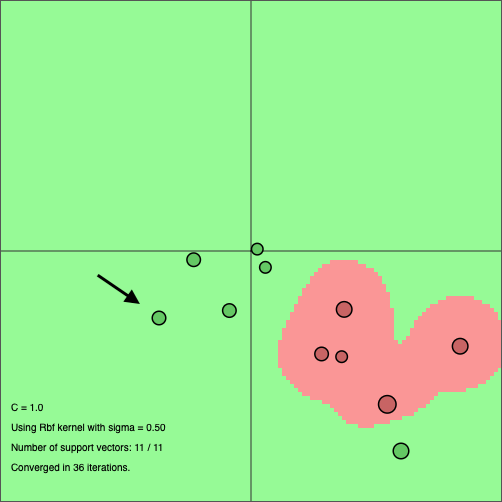
\includegraphics[width=0.17\textwidth]{../src/figures/stanford/canvasnewrbf3}}\\
\subfloat[Modelling the \texttt{XOR} function ($\sigma^2=0.1$).]{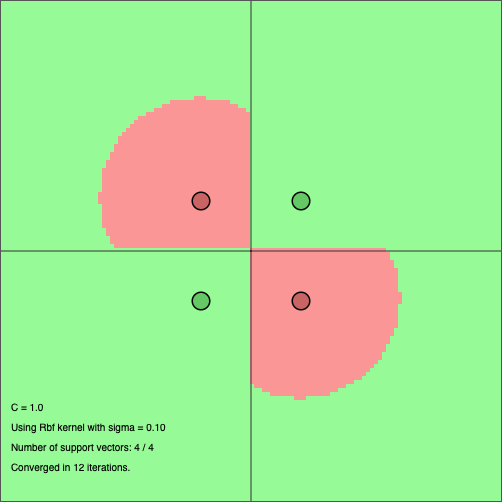
\includegraphics[width=0.17\textwidth]{../src/figures/stanford/canvasxor3}}\qquad
\subfloat[Modelling the \texttt{XOR} function ($\sigma^2=100$).]{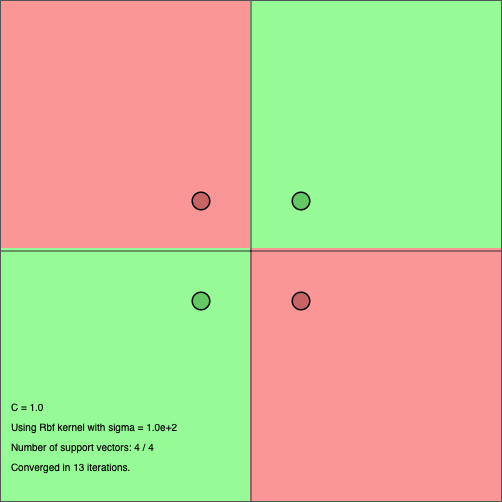
\includegraphics[width=0.17\textwidth]{../src/figures/stanford/canvasxor}}\qquad
\subfloat[Same as the left two pictures with another data point belonging to the positive class.]{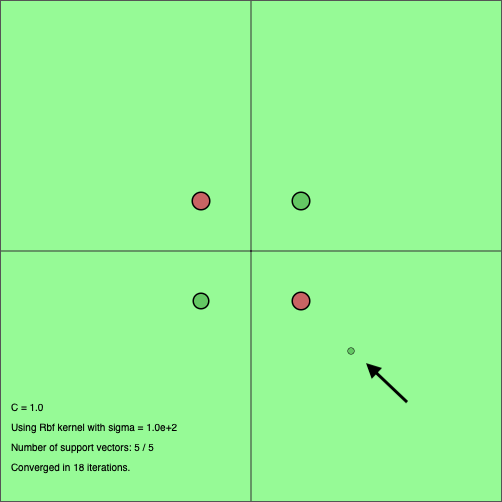
\includegraphics[width=0.17\textwidth]{../src/figures/stanford/canvasxor2}}\\
\caption{Visualisation of various experiments with $C$ (top row), addition of points using the linear kernel (second row), $\sigma$ (third row), addition of points using the RBF kernel (fourth row) and the $\texttt{XOR}$ function (last row). The number of iterations (tends to) increase as $C$ gets larger or as the number of data points increases.}
\label{stanfordexample}
\end{figure}
\clearpage

\par\noindent For the given toy dataset it can readily be seen in figure \ref{stanfordexample} (top row) that for a decreasing value of $C$ the margin does become larger and that less \textit{`slacking'} is allowed for. By adding data points close to the boundary or at the \textit{`wrong'} side of it the margin usually changes a lot and the new data points nearly always become support vectors.

The $\sigma^2$ hyperparameter in the case of an RBF kernel controls the locality of each data point. As it increases the feature space mapping becomes smoother, producing simpler decision boundaries (figure \ref{stanfordexample}, third row). This relates to the bias-variance tradeoff. For $\sigma^2$ small enough any two classes get separated in a very strict way - the Gaussian kernels are universal. For very large bandwidths the reach of each data point becomes large and the decision boundary become near-linear as the density areas of each class end up competing and the problem reduces to something similar to what's seen in the introductory example\footnote{When the demo is run on a 4-point dataset representing the \texttt{XOR} function a checkerboard pattern is obtained when $\sigma^2$ is large (as seen in figure \ref{stanfordexample}, last row). Even when $\sigma^2$ is low the separation is linear in between the data points as the problem reduces to that seen in the introductory example.}. As for $C$, it works the same as before, prioritising either larger margins or lower misclassification rates. When $\sigma^2$ is large a bigger value of $C$ can make the model more complex again. 

\par\noindent The RBF kernel approach can generate models having misclassification rates that are lower than the classic linear kernel approach does as decision boundaries that are nonlinear in the input space can be learned. It also tends to use more data points as support vectors. This makes the model less compact (computationally efficient) and if the data is linearly separable it is unnecessary. Deciding whether the model generalises better can be done through evaluation on a test set.

\fakesubsection{Least-squares support vector machine classifier}{}

Figure \ref{iris} depicts results on the iris dataset using various polynomial kernels with $t=1$. This $t$ is called the \textit{constant} and it controls the importance of higher - versus lower-order terms in the polynomial as can be deduced from the application of the binomial theorem to the definition of the kernel :
$$(x^T\cdot y+\tau)^d=\sum_{i=0}^d\binom{d}{i}(x^T\cdot y)^{d-i}\cdot \tau^i$$
The effect of $t$ is not very noticeable for small values of $d$ while for the higher degrees it tends to make the decision boundary more complex.

\par\noindent When the degree $\delta$ is 1 the feature map is linear which is equivalent to the classic non-linear SVM problem while for higher degrees a boundary of increasing complexity is learned such that for $\delta\in\{3,4\}$ no data points are misclassified. To make it less likely that the model overfits a lower $\delta$ is likely to be preferable (this corresponds to the application of Occam's razor).

%\begin{figure}[h]
%\centering
%\subfloat[$\gamma=0.1,\delta=1,\rho=0.5$]{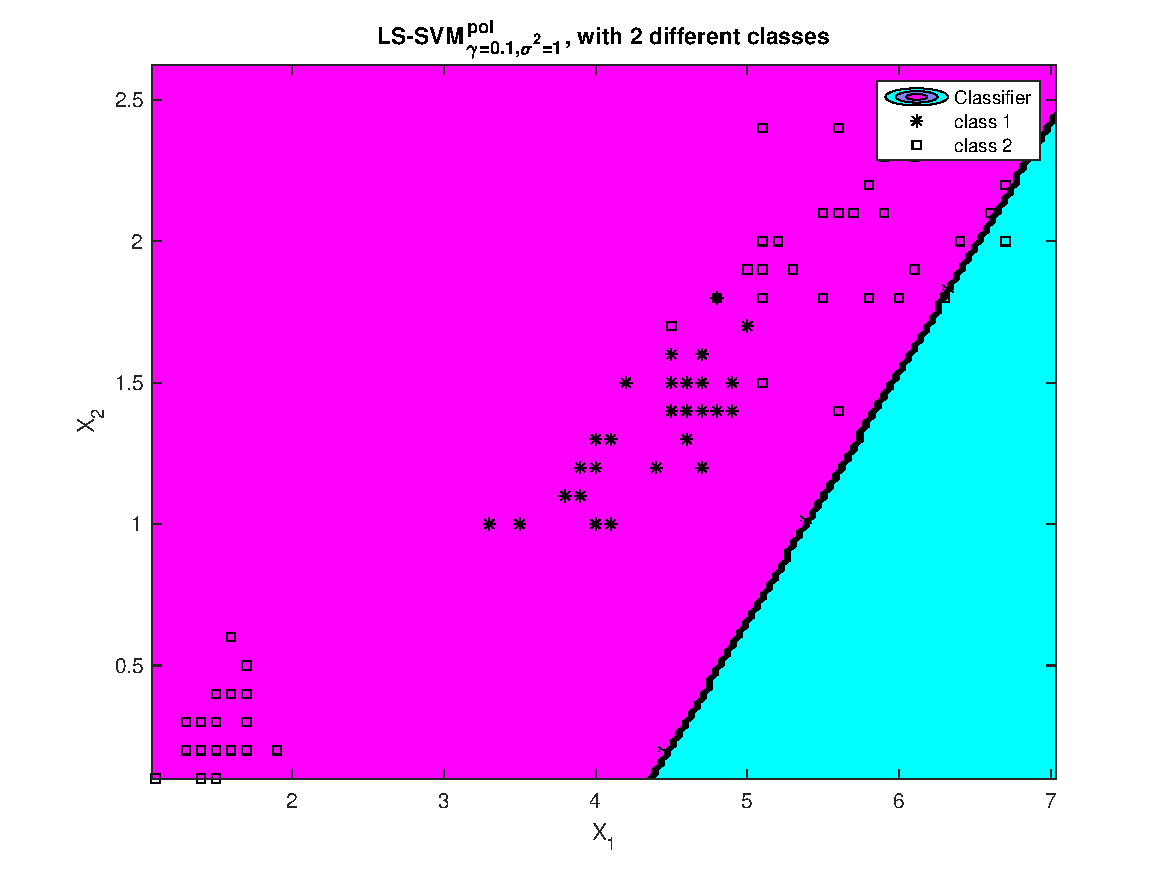
\includegraphics[width=0.3\textwidth]{../src/figures/iris/t=1/1_1}}\qquad
%\subfloat[$\gamma=1.0,\delta=1,\rho=0.55$]{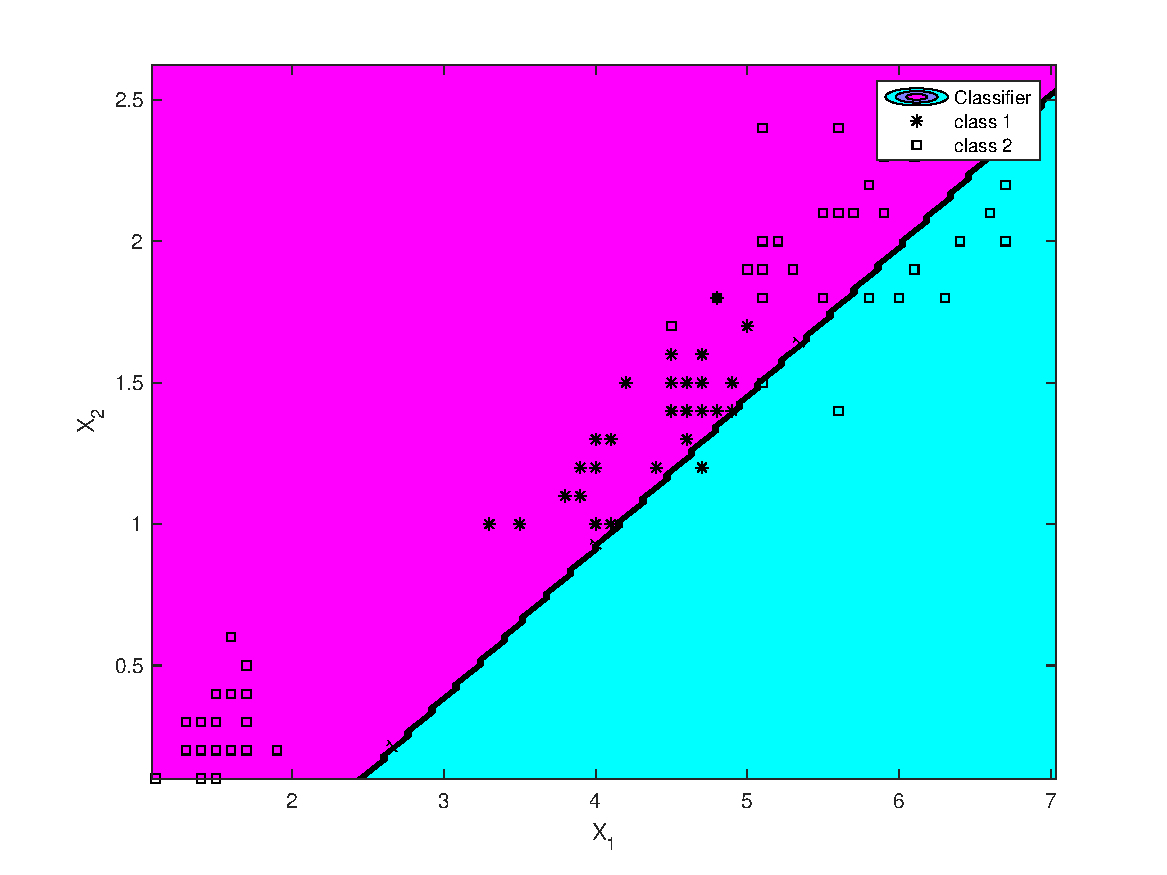
\includegraphics[width=0.3\textwidth]{../src/figures/iris/t=1/1_10}}\qquad
%\subfloat[$\gamma=10.0,\delta=1,\rho=0.55$]{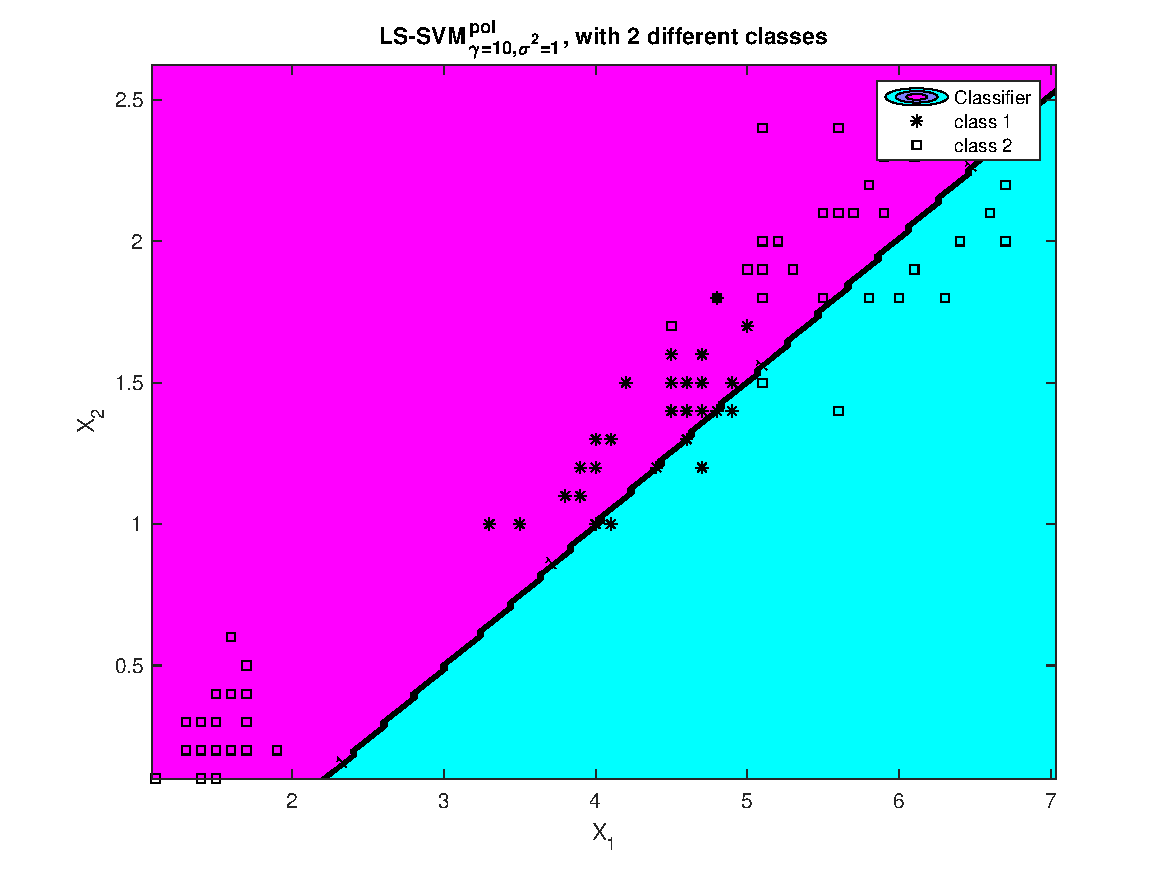
\includegraphics[width=0.3\textwidth]{../src/figures/iris/t=1/1_100}}\qquad
%\\
%\subfloat[$\gamma=0.1,\delta=2,\rho=0.05$]{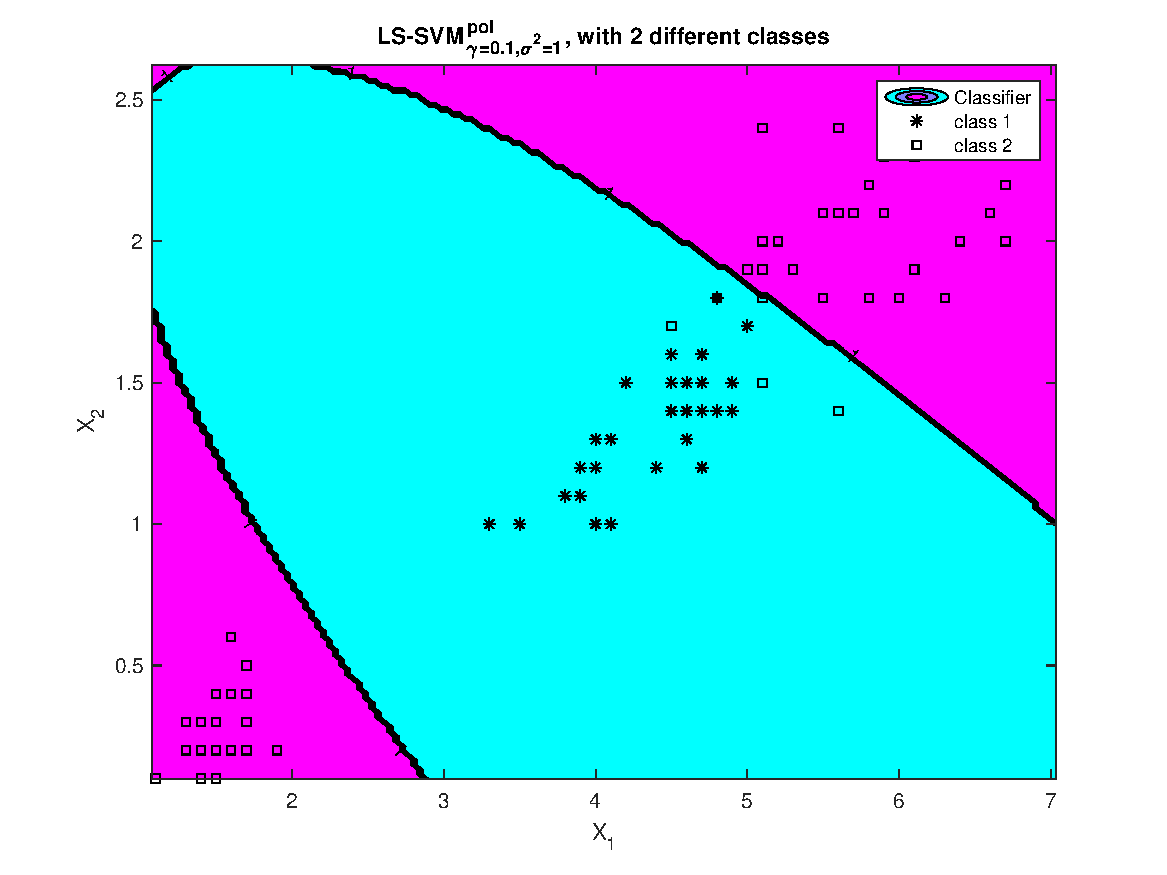
\includegraphics[width=0.3\textwidth]{../src/figures/iris/t=1/2_1}}\qquad
%\subfloat[$\gamma=1.0,\delta=2,\rho=0.05$]{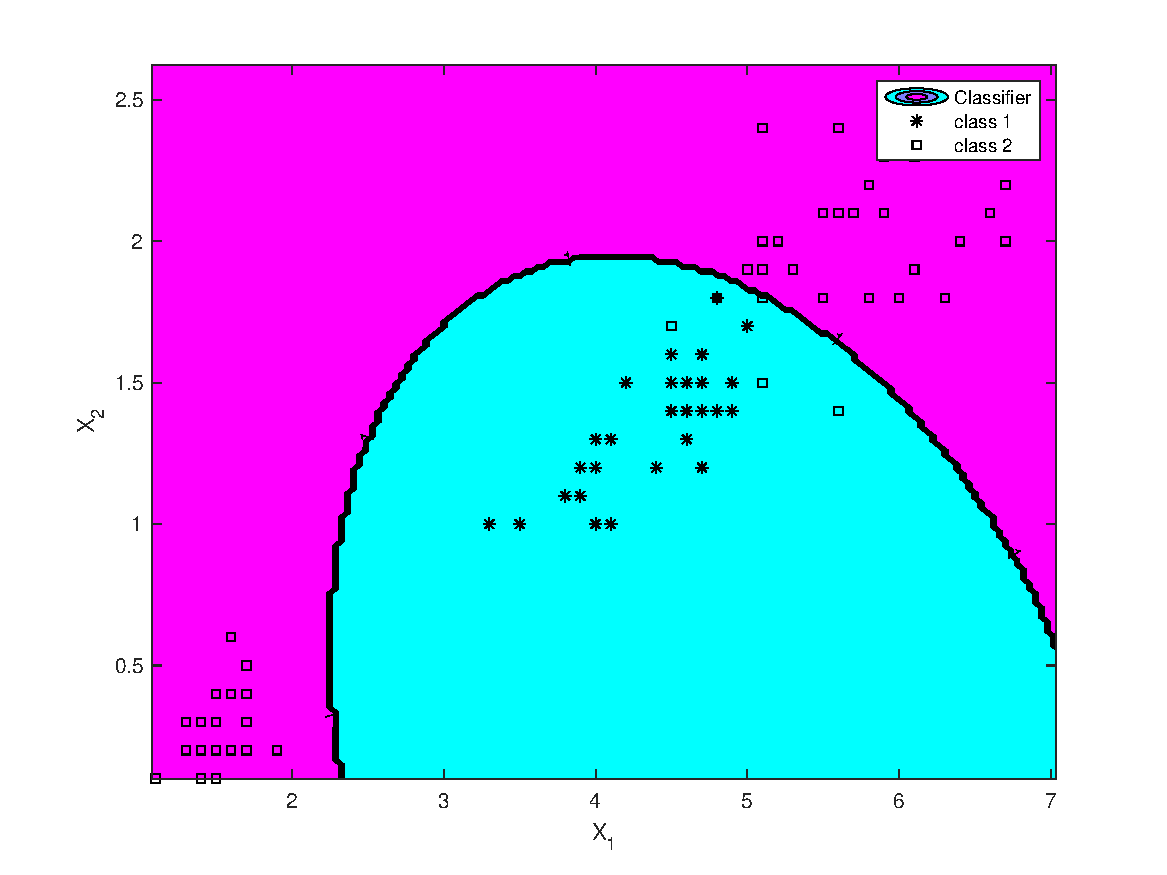
\includegraphics[width=0.3\textwidth]{../src/figures/iris/t=1/2_10}}\qquad
%\subfloat[$\gamma=10.0,\delta=2,\rho=0.05$]{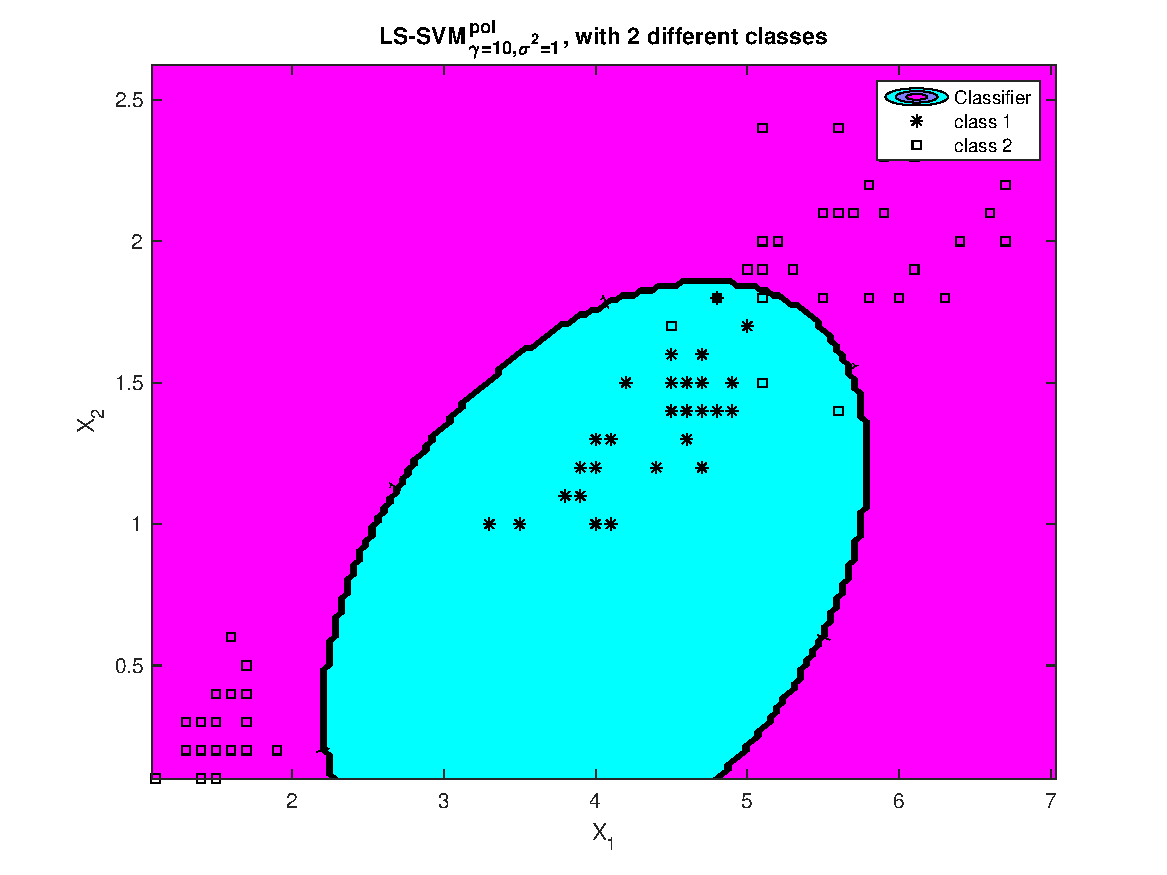
\includegraphics[width=0.3\textwidth]{../src/figures/iris/t=1/2_100}}\qquad
%\\
%\subfloat[$\gamma=0.1,\delta=3,\rho=0.0$]{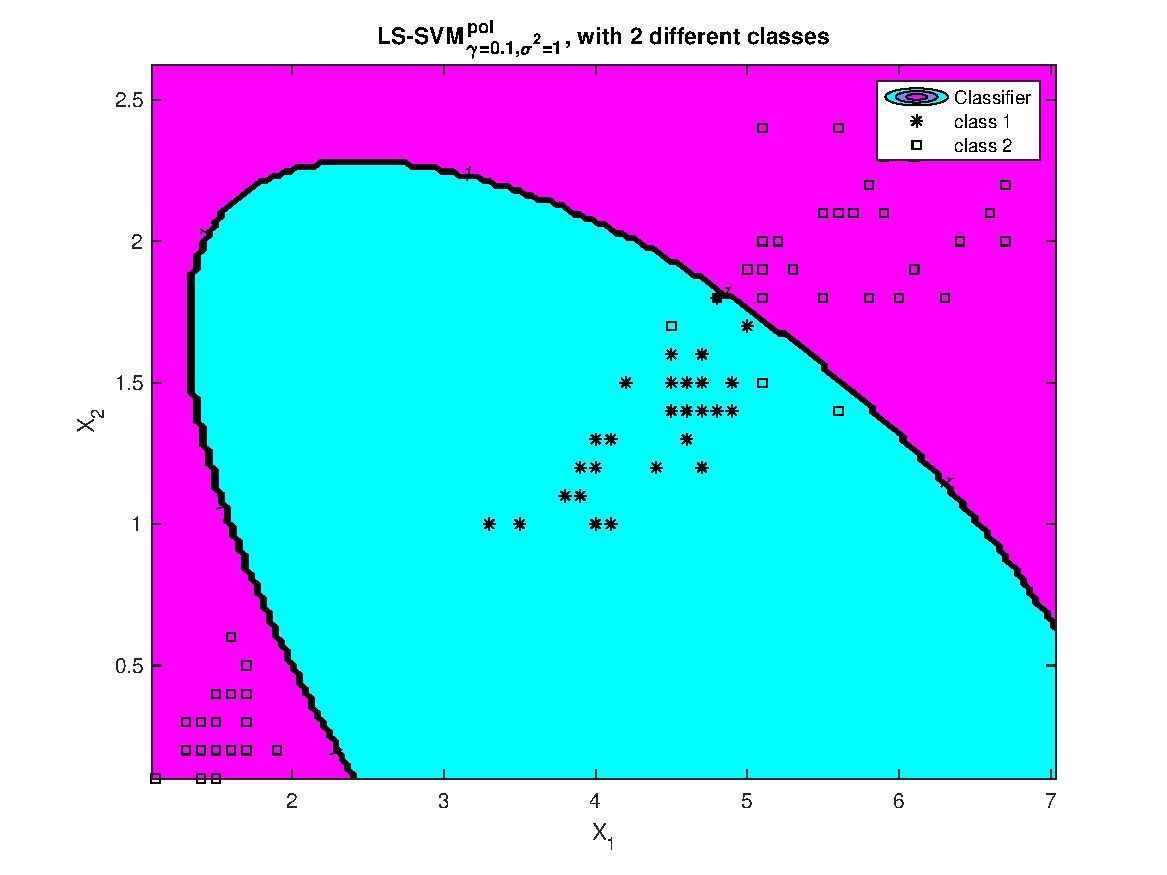
\includegraphics[width=0.3\textwidth]{../src/figures/iris/t=1/3_1}}\qquad
%\subfloat[$\gamma=1.0,\delta=3,\rho=0.0$]{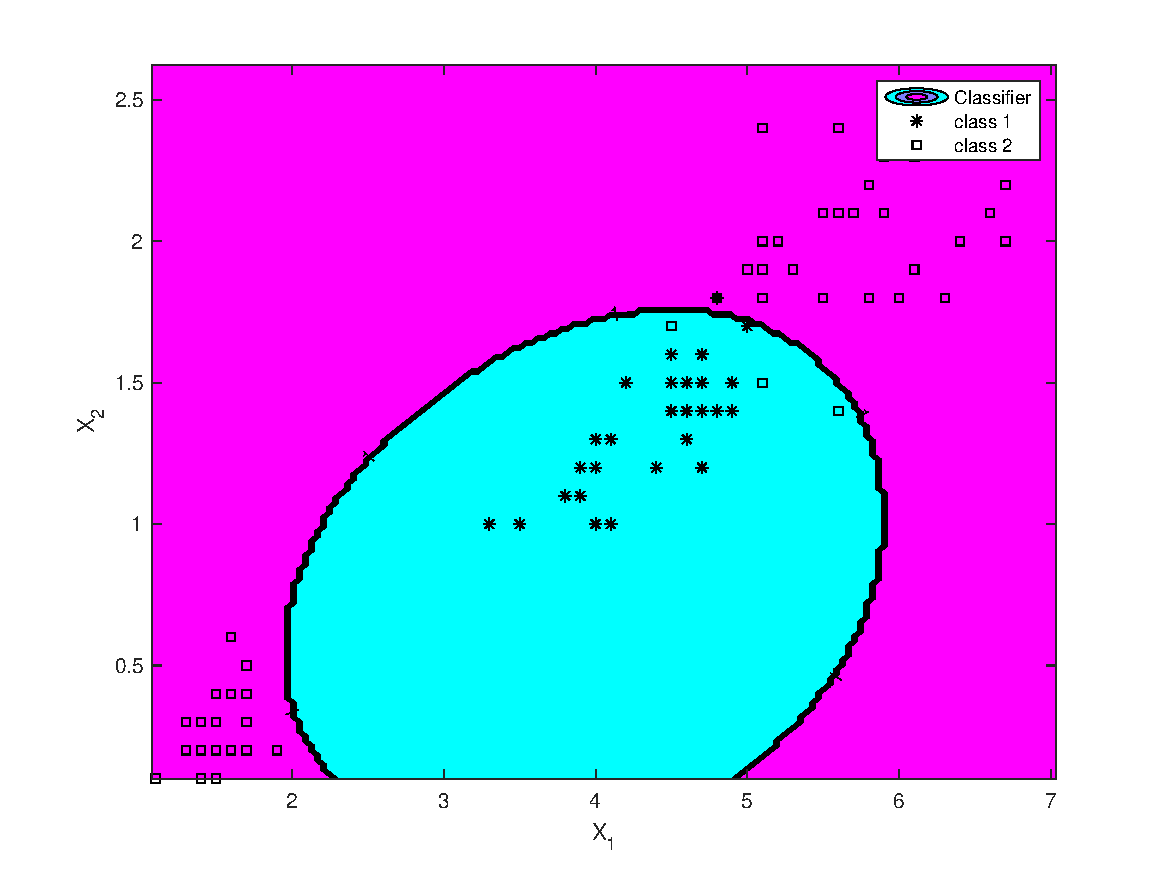
\includegraphics[width=0.3\textwidth]{../src/figures/iris/t=1/3_10}}\qquad
%\subfloat[$\gamma=10.0,\delta=3,\rho=0.0$]{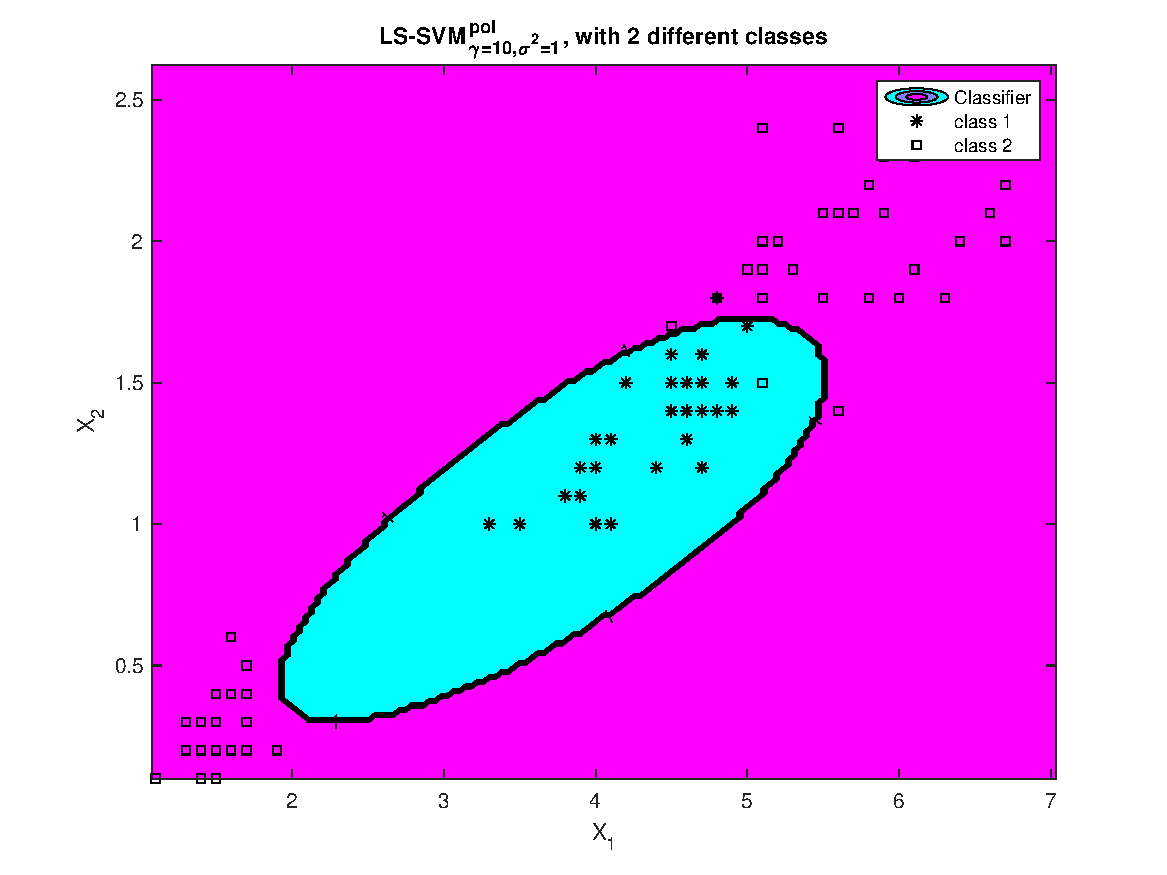
\includegraphics[width=0.3\textwidth]{../src/figures/iris/t=1/3_100}}\qquad
%\\
%\subfloat[$\gamma=0.1,\delta=4,\rho=0.0$]{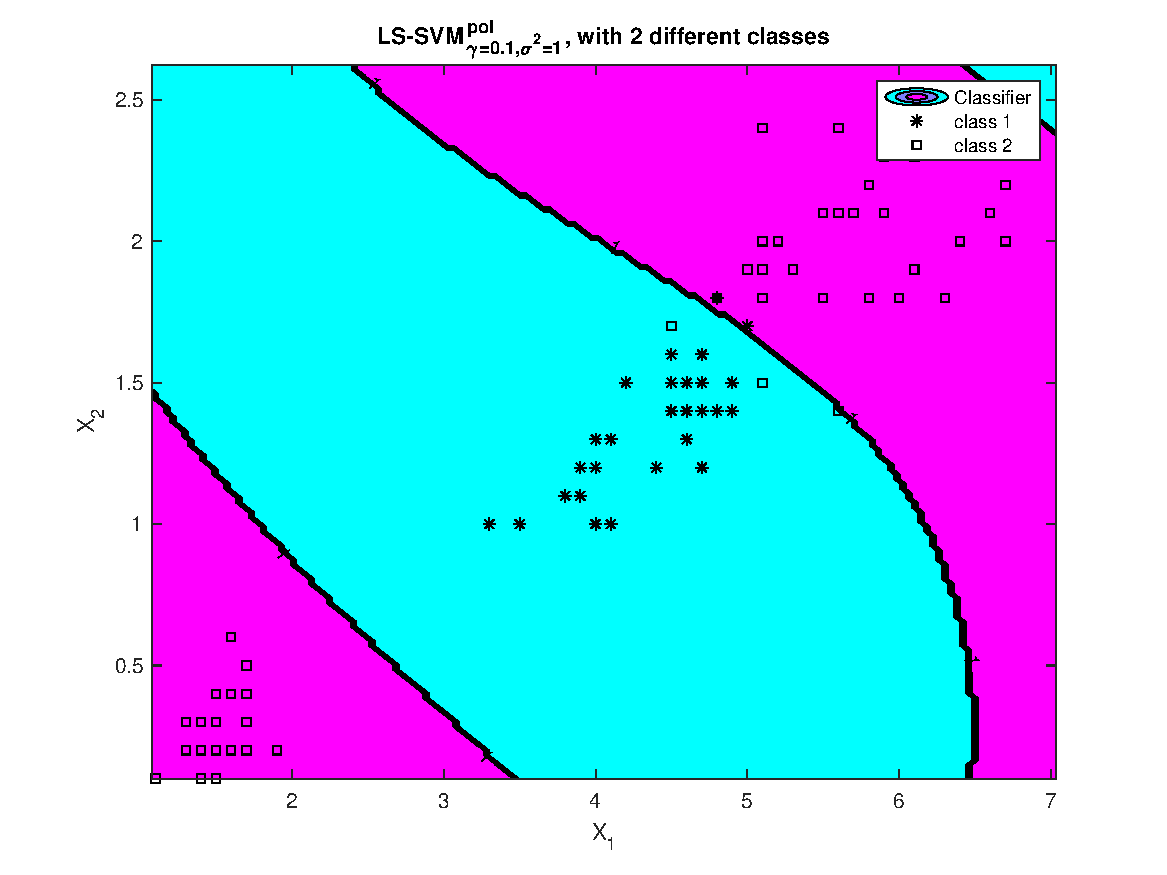
\includegraphics[width=0.3\textwidth]{../src/figures/iris/t=1/4_1}}\qquad
%\subfloat[$\gamma=1.0,\delta=4,\rho=0.0$]{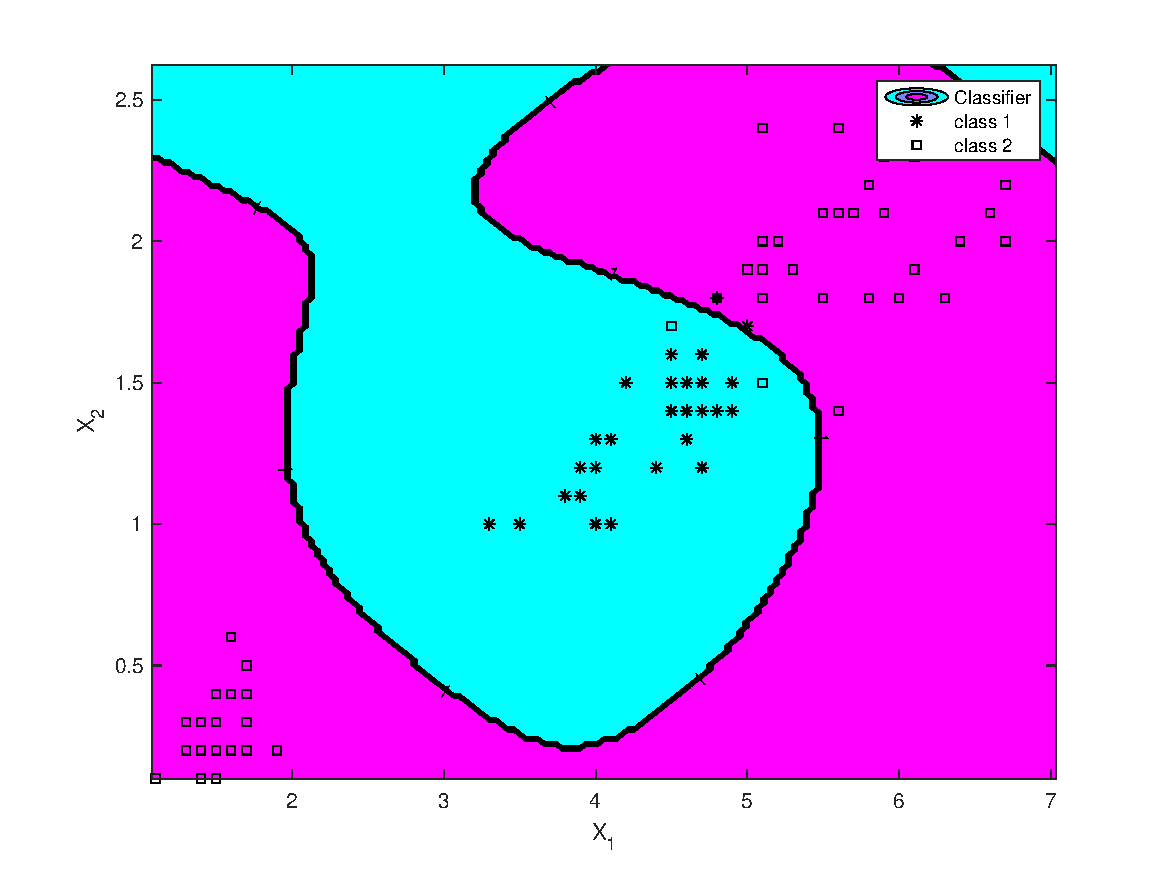
\includegraphics[width=0.3\textwidth]{../src/figures/iris/t=1/4_10}}\qquad
%\subfloat[$\gamma=10.0,\delta=4,\rho=0.0$]{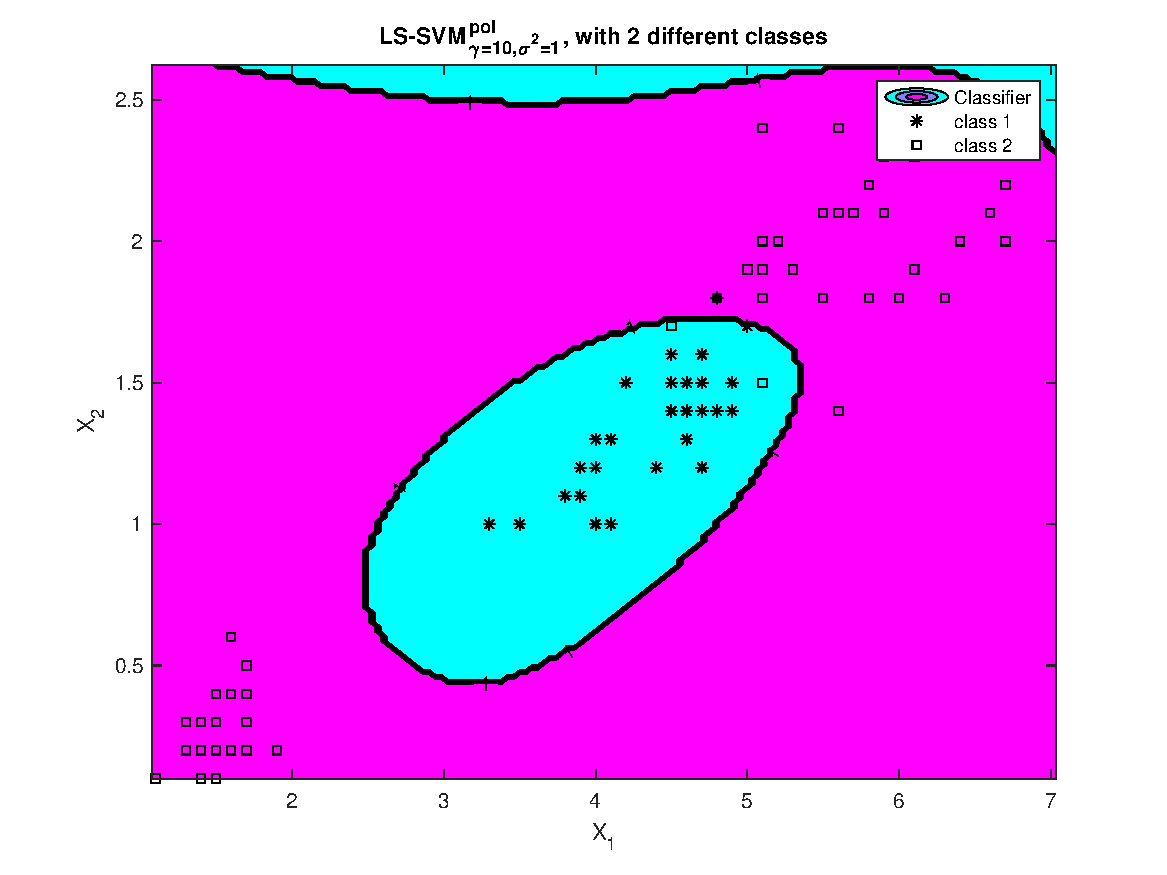
\includegraphics[width=0.3\textwidth]{../src/figures/iris/t=1/4_100}}
%\caption{Visualisation of the results of experiments with polynomial kernels on the iris dataset ($\delta$ is the degree of the polynomial, $\rho$ the misclassification rate on the test set, $t$ is fixed to 1). As the degree of the kernel increases, the misclassification error drops.}
%\end{figure}

\vspace{-0.5cm}
\begin{figure}[htp]
\centering
\subfloat[$\delta=1,\rho=0.55$]{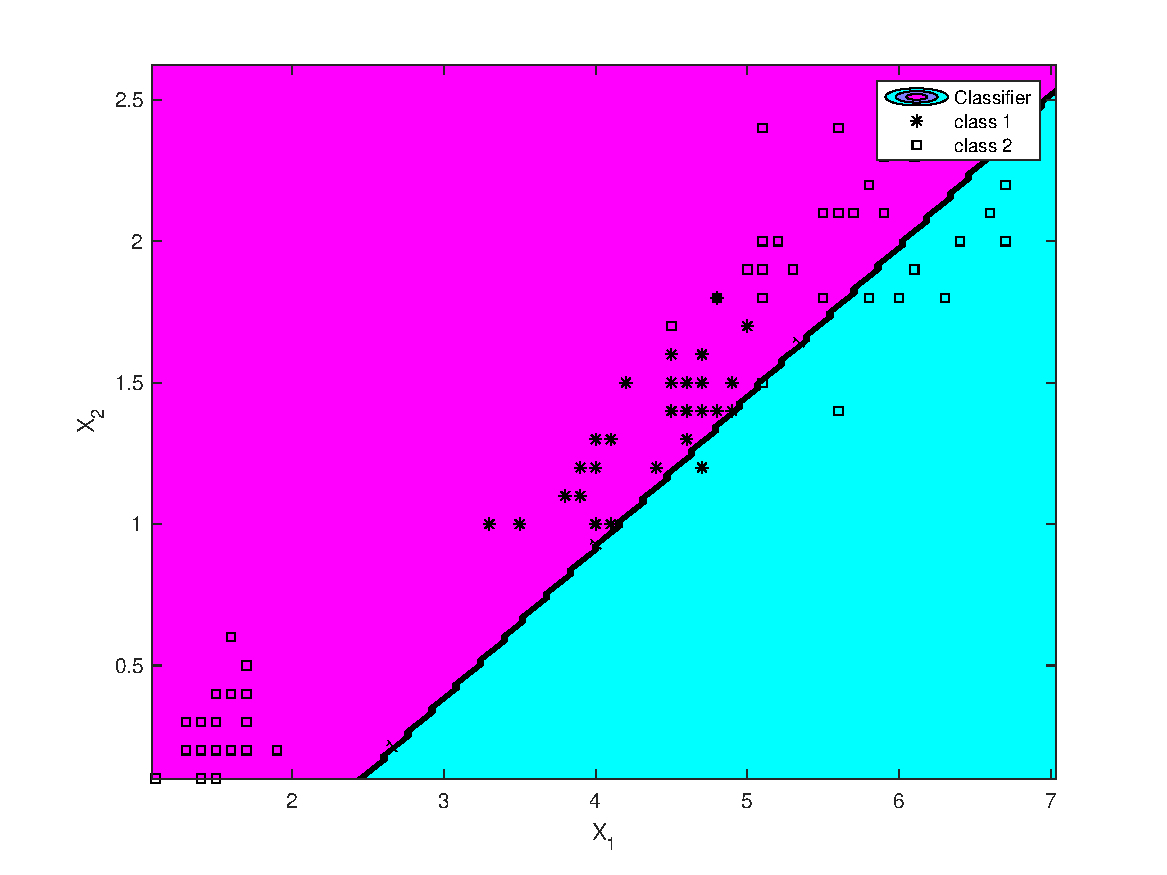
\includegraphics[width=0.25\textwidth]{../src/figures/iris/t=1/1_10}}\hfil
\subfloat[$\delta=2,\rho=0.05$]{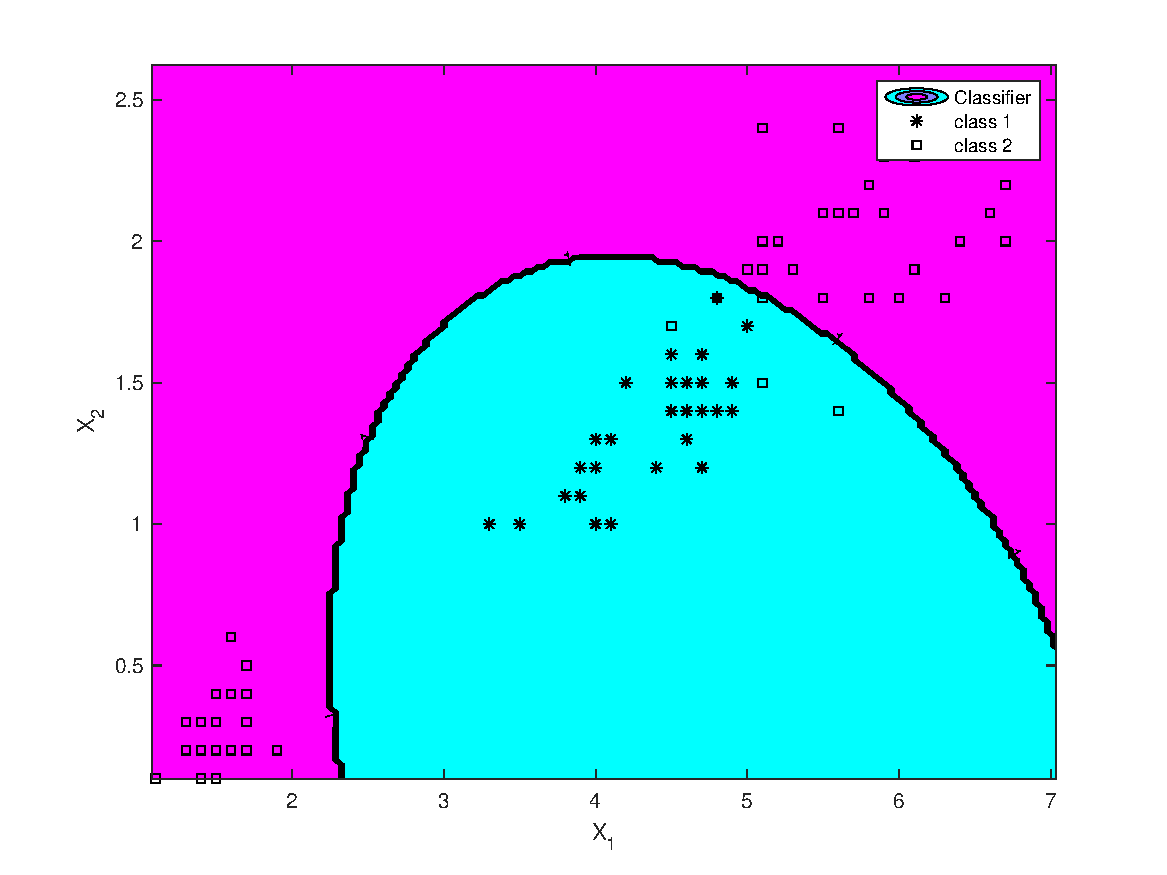
\includegraphics[width=0.25\textwidth]{../src/figures/iris/t=1/2_10}}\hfil
\subfloat[$\delta=3,\rho=0.0$]{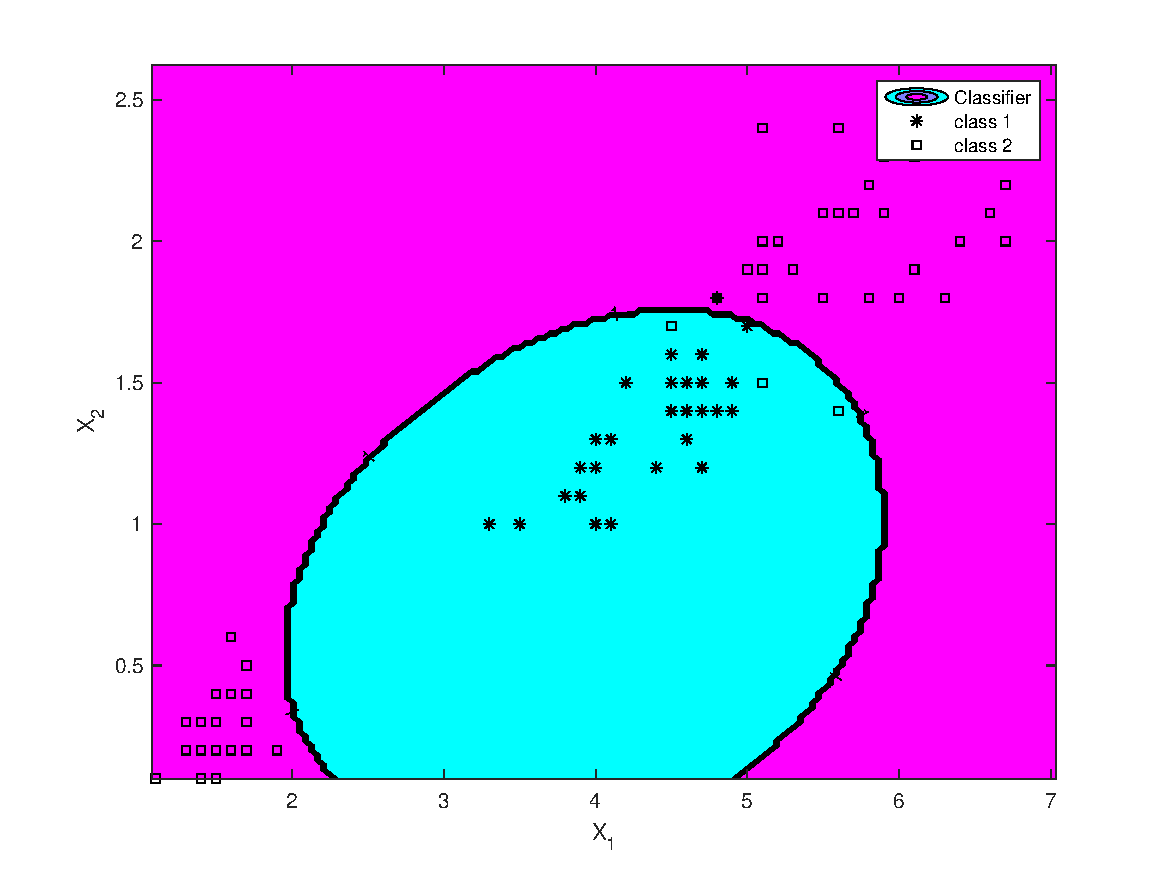
\includegraphics[width=0.25\textwidth]{../src/figures/iris/t=1/3_10}}\hfil
\subfloat[$\delta=4,\rho=0.0$]{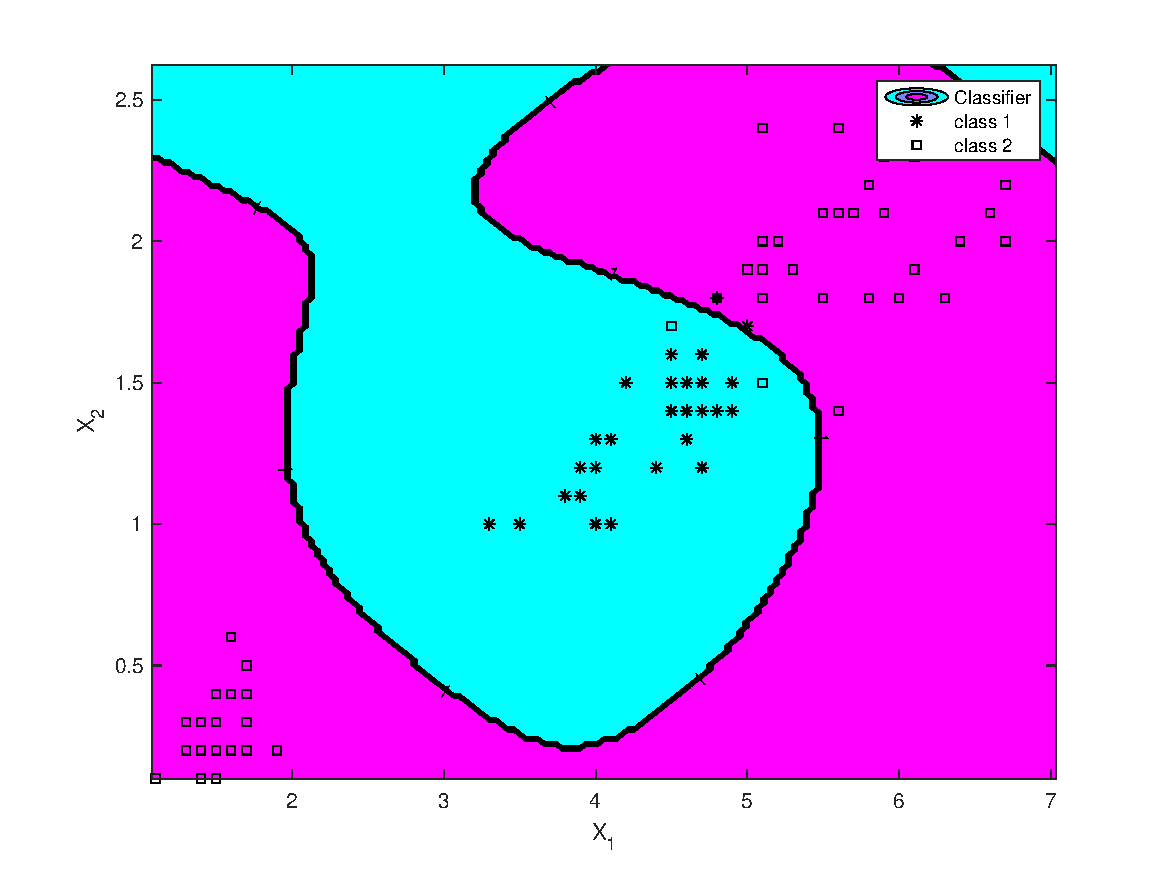
\includegraphics[width=0.25\textwidth]{../src/figures/iris/t=1/4_10}}\hfil
\caption{Visualisation of the results of experiments with polynomial kernels on the iris dataset ($\delta$ is the degree of the polynomial, $\rho$ the misclassification rate on the test set, $t$ is fixed to 1). As the degree of the kernel increases, the misclassification error drops.}
\label{iris}
\end{figure}

\par In the case of RBF kernels one can see in figure \ref{iris2} that for a $\gamma$ value of 1 any $\sigma^2$ between 0.1 and 1 performs well. The same interval works for $\gamma$ when $\sigma^2=1$. This corresponds to the results of the provided sample script where the base used in the semilog plot happens to be the natural logarithm (instead of using base 10). For large $\sigma$ values (say, 25) one class may overtake the other one. The experiment is of limited value as only few parameter combinations were tried.

\par To properly find good parameter values a more systematic approach is in order. The idea is to search through the parameter space and evaluate the results on a validation set rather than on the test set (which should be used for nothing but the evaluation of the finished model). A validation set can be constructed in a few ways the results of which are illustrated in figure \ref{validation}, where error estimates in the parameter space are shown. Random splitting i.e. splitting the input data randomly in a training - and a validation set is a way that isn't particularly robust. An improvement upon it is $k$-fold validation where the input data is randomly split into $k$ folds which are considered as a validation set in turn such that all the input data can be used for parameter tuning. When $k=N$ with $N$ the number of input samples this is called leave-one-out cross-validation. 

\begingroup
\setlength{\columnsep}{0.75cm}
\setlength{\intextsep}{0.2cm}
\begin{wrapfigure}{r}{0pt}
\centering
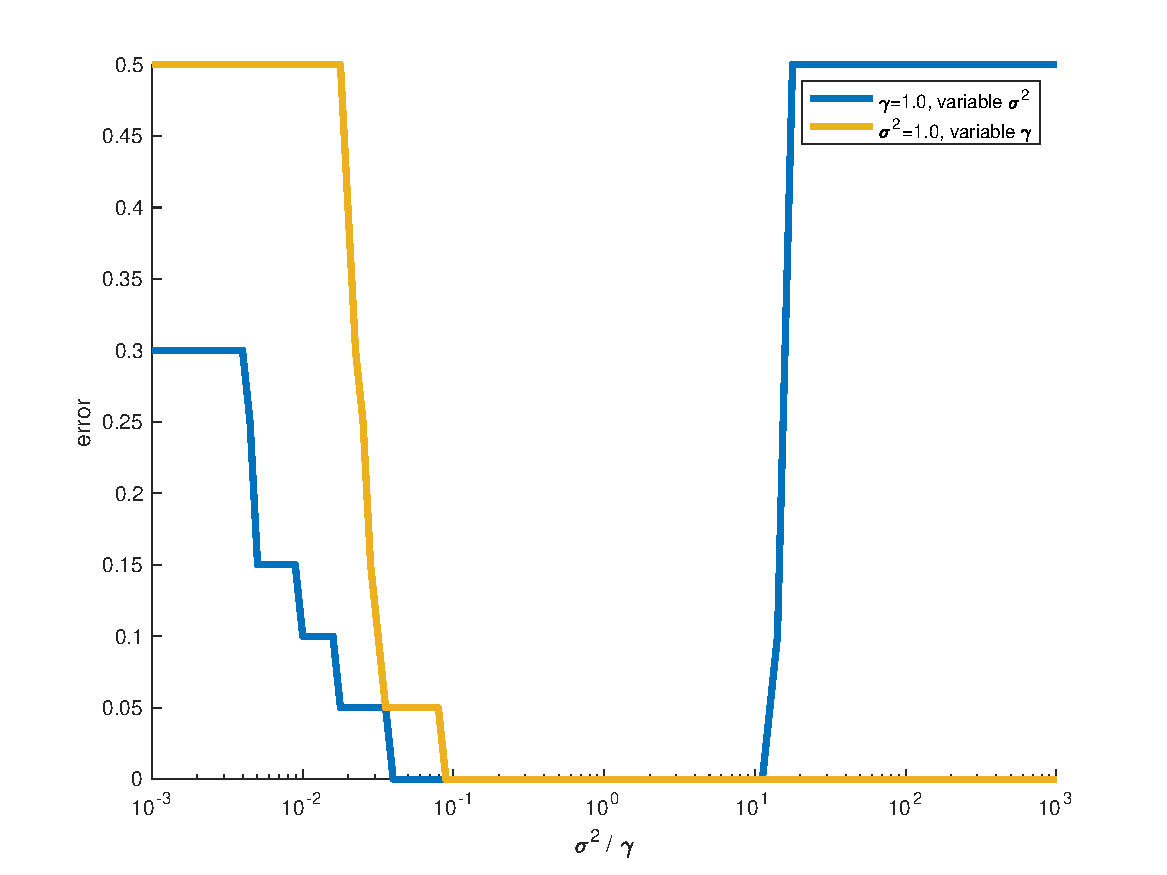
\includegraphics[width=0.45\textwidth]{../src/figures/iris/tuning}
\caption{Performance of various RBF kernels on the iris dataset. The orange curve denotes the performance of the model for varying $\gamma$ and fixed $\sigma^2=1.0$, the blue curve does the opposite ($\gamma=1.0$, varying $\sigma^2$).}
\label{iris2}
\end{wrapfigure}

\par To some extent deciding what $k$ value to use parallels previous discussions about other parameters since there's a bias-variance tradeoff ; while larger $k$ values should provide a better estimate of the error they also suffer from higher variance as the result depends more on how representative the input data is. This becomes more important when the number of input data is small. Finally, $k$ shouldn't be too small (such that the training sets remain large enough), it should preferably be a divisor of $N$ (though this is not of primary importance) and if computational expense is an issue it cannot be large as many models would have to be generated.

\par Automated tuning uses these validation methods in conjunction with a search procedure to find useful combinations of parameters. This search strategy has to deal with a non-convex problem and can be a simple grid search (performing validation for every combination of parameters specified by a grid partitioning the parameter space) or the Nelder-Mead method. The latter aims to find the minimum of a function without needing its derivative by considering a simplex which is updated iteratively until it wraps around the minimum. It tends to execute faster than grid search especially when the number of parameters is high, though to address this one could also consider a variant of grid search that starts with a grid of limited granularity until it finds a promising region in the parameter space on which grid search is performed again.

\endgroup

\par In the LS-SVM toolbox a technique called \textit{coupled simulated annealing} is used. This is a global optimisation technique which couples together several simulated annealing processes (inspired by coupled local minimisers' effectiveness compared to multi-start gradient descent optimisation). Its output is subsequently provided to either a grid search - or a Nelder-Mead algorithm. Results are the following :

\begin{table}[h]
\centering
\begin{tabular}{c|ccc}
\textit{Method} & $\gamma$ & $\sigma^2$ & \textit{cost} \\
\hline
Grid search & 16983.8488 $\pm$ 100324.6730 & 10.5373 $\pm$ 83.0560 & 0.0339 $\pm$ 0.0063\\
Nelder-Mead & 85111.5137 $\pm$ 75855.5677 & 12.8189 $\pm$ 71.4858 & 0.0349 $\pm$ 0.0069\\
\end{tabular}
\caption{Results of automated tuning strategies (averaged over 100 runs).}
\label{automatedtuning}
\end{table}

Simulated annealing is a stochastic process such that the parameters end up varying quite a bit. The costs do not since they are minimised. A histogram of the results gives a more complete picture and shows that there are a few outliers that make the average $\gamma$ and $\sigma^2$ large :

\begin{figure}[h]
\centering
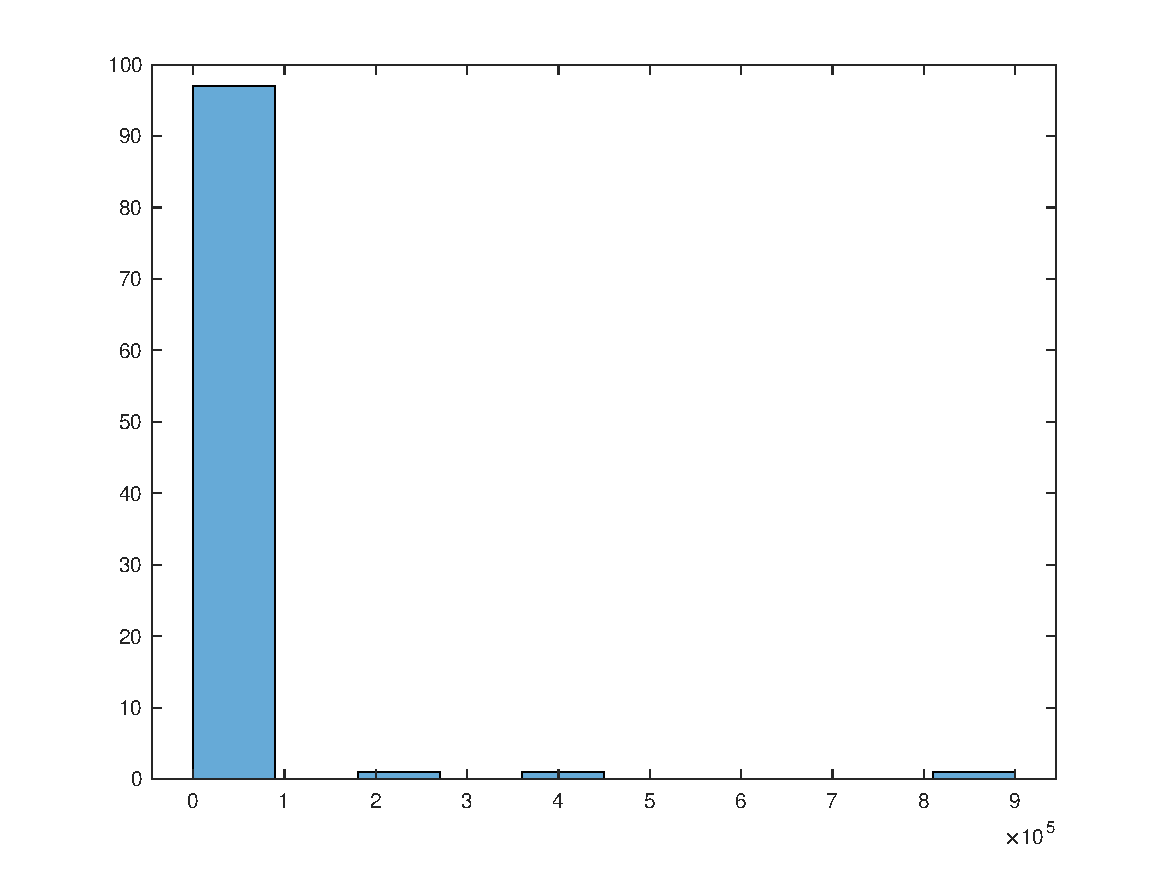
\includegraphics[width=0.25\textwidth]{../src/figures/iris/histogram_gamma}\quad
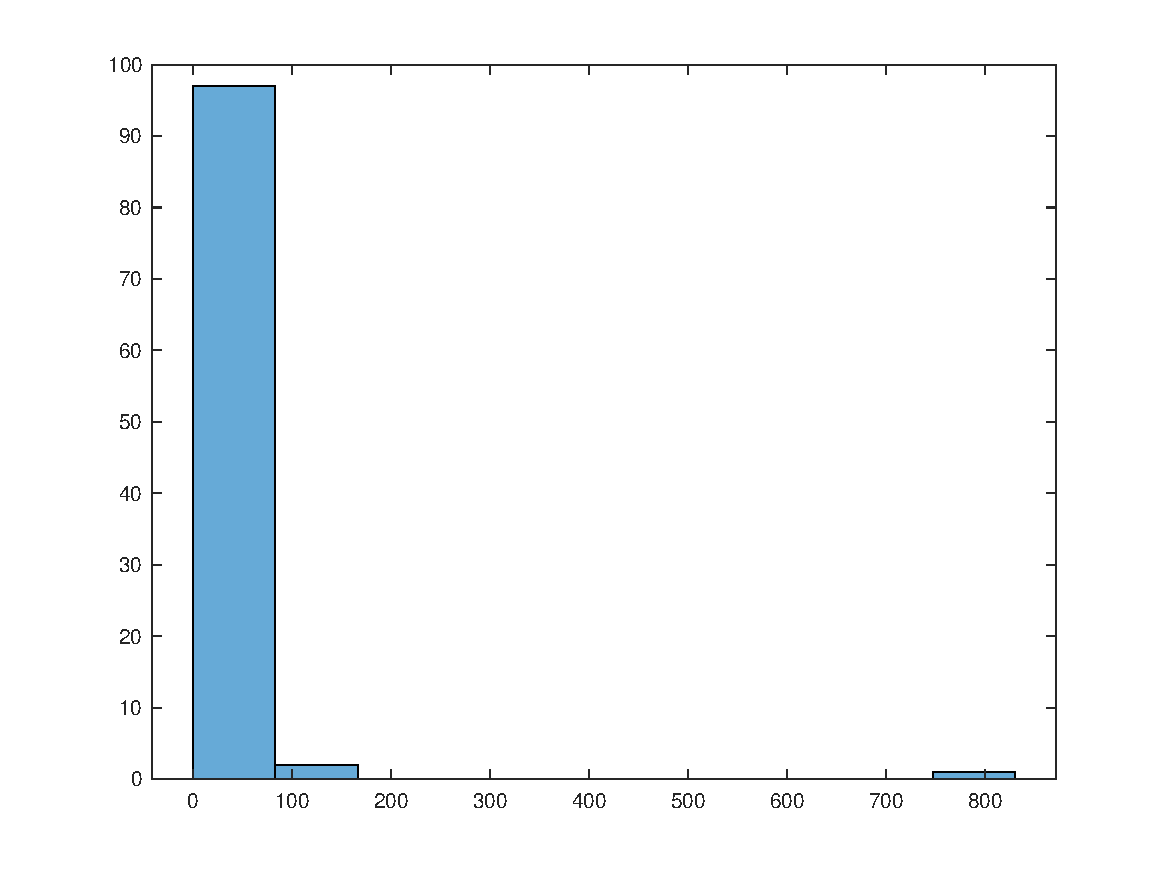
\includegraphics[width=0.25\textwidth]{../src/figures/iris/histogram_sigma2}\quad
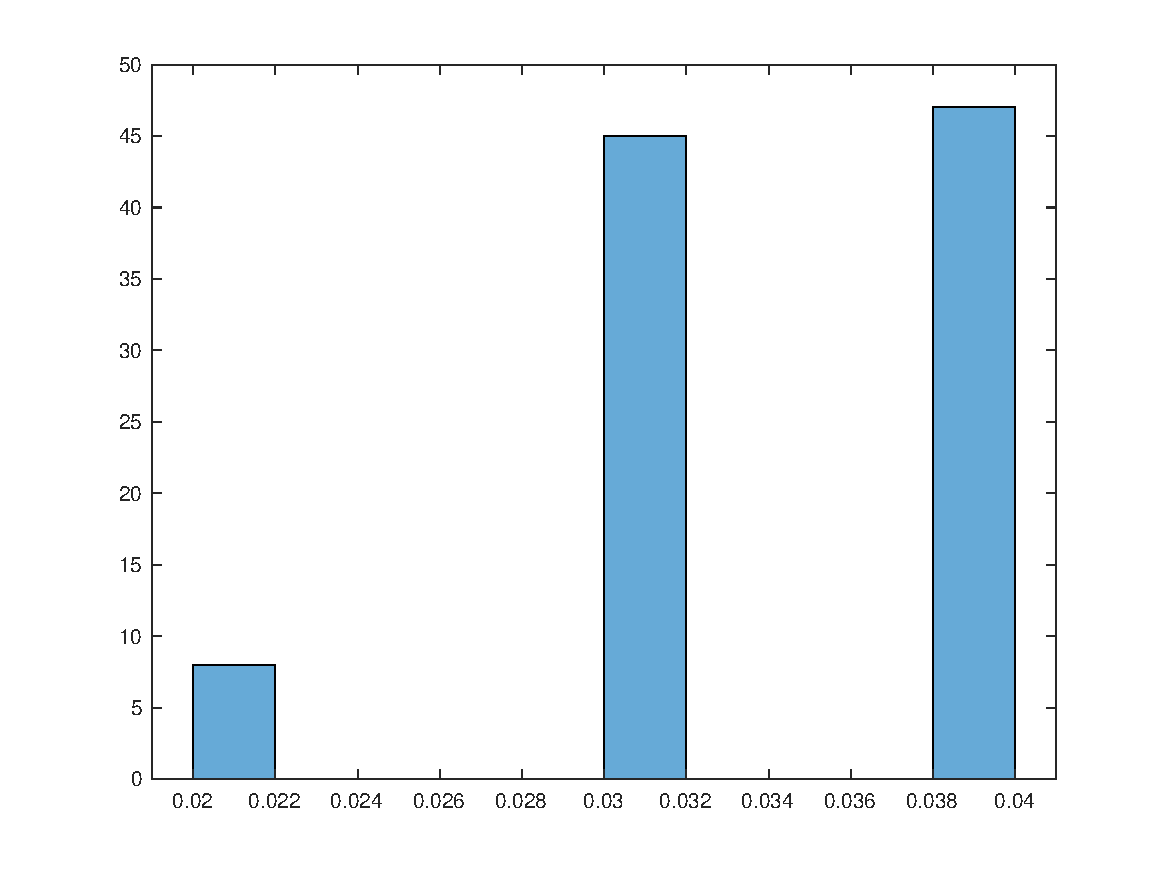
\includegraphics[width=0.25\textwidth]{../src/figures/iris/histogram_cost}
\caption{Histograms for 100 $\gamma$, $\sigma^2$ and costs returned by the automated tuning process.}
\label{automatedtuninghistogram}
\end{figure}

Results of the automated tuning process correspond to the contour plots given in figure \ref{validation}. As for the runtimes, the grid search ended up being twice as slow as the simplex method.

%\begingroup
%\setlength{\columnsep}{0.75cm}
%\setlength{\intextsep}{0cm}
%\begin{wrapfigure}{l}{0pt}
%\centering
%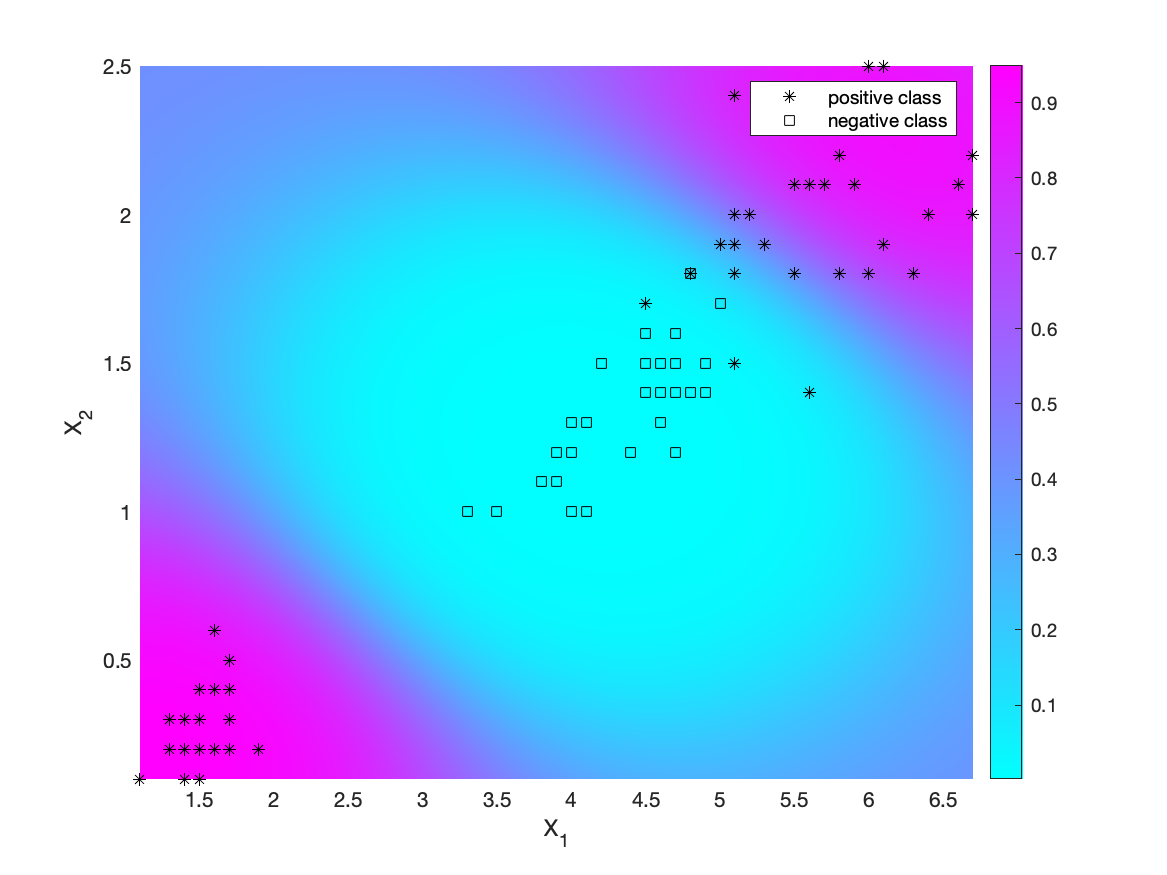
\includegraphics[width=0.45\textwidth]{../src/figures/iris/bayesian/bayesian_probabilities}
%\caption{Posterior probability estimates using a Bayesian approach ($\gamma\approx0.038,\sigma^2\approx 0.56$). The hue indicates the probability that the data point at a location in the 2-dimensional plane belongs to one or the other class. A smaller $\sigma^2$ can lead to overfitting and makes for a more clearly defined, smaller blue area.}
%\label{irisbayesian}
%\end{wrapfigure}

\begin{figure}[htp]
\centering
\subfloat[Random split validation.]{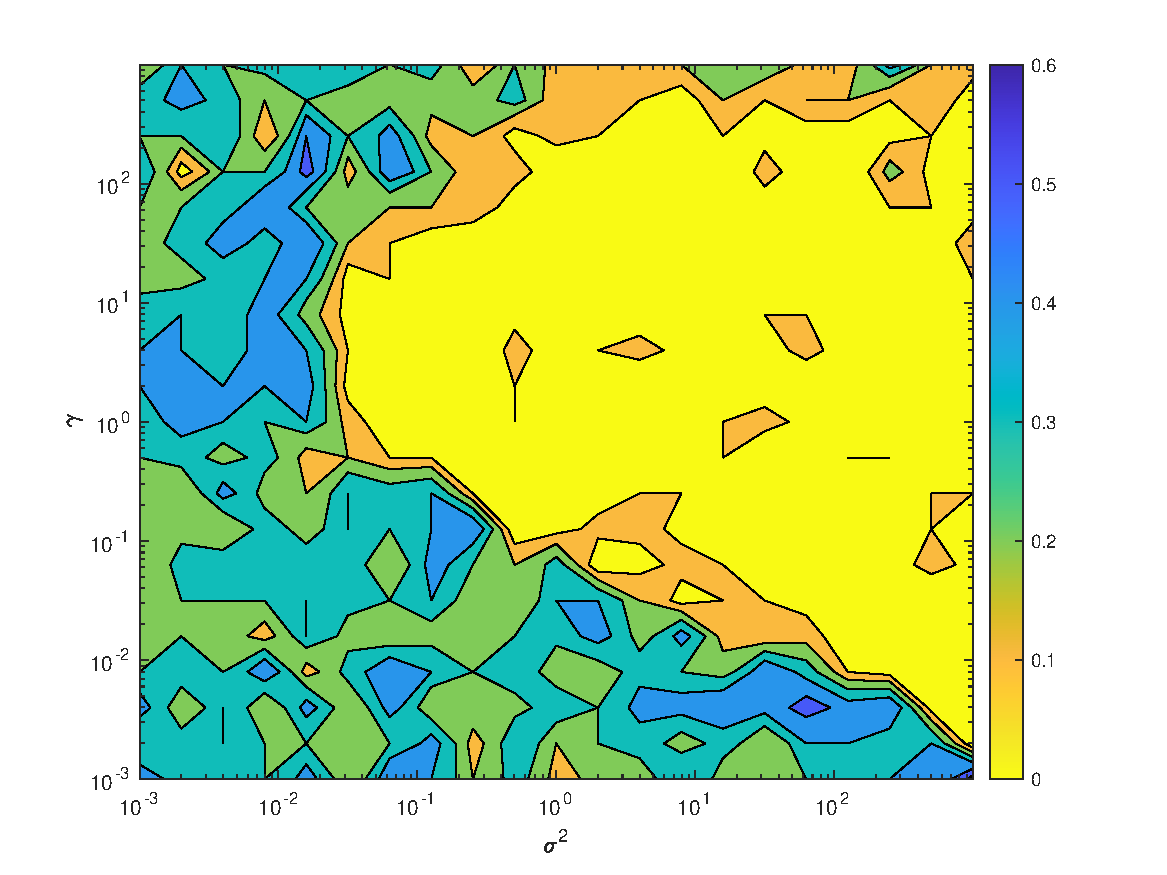
\includegraphics[width=0.33\textwidth]{../src/figures/iris/validation_1}}\hfil
\subfloat[$k$-fold validation ($k=10$).]{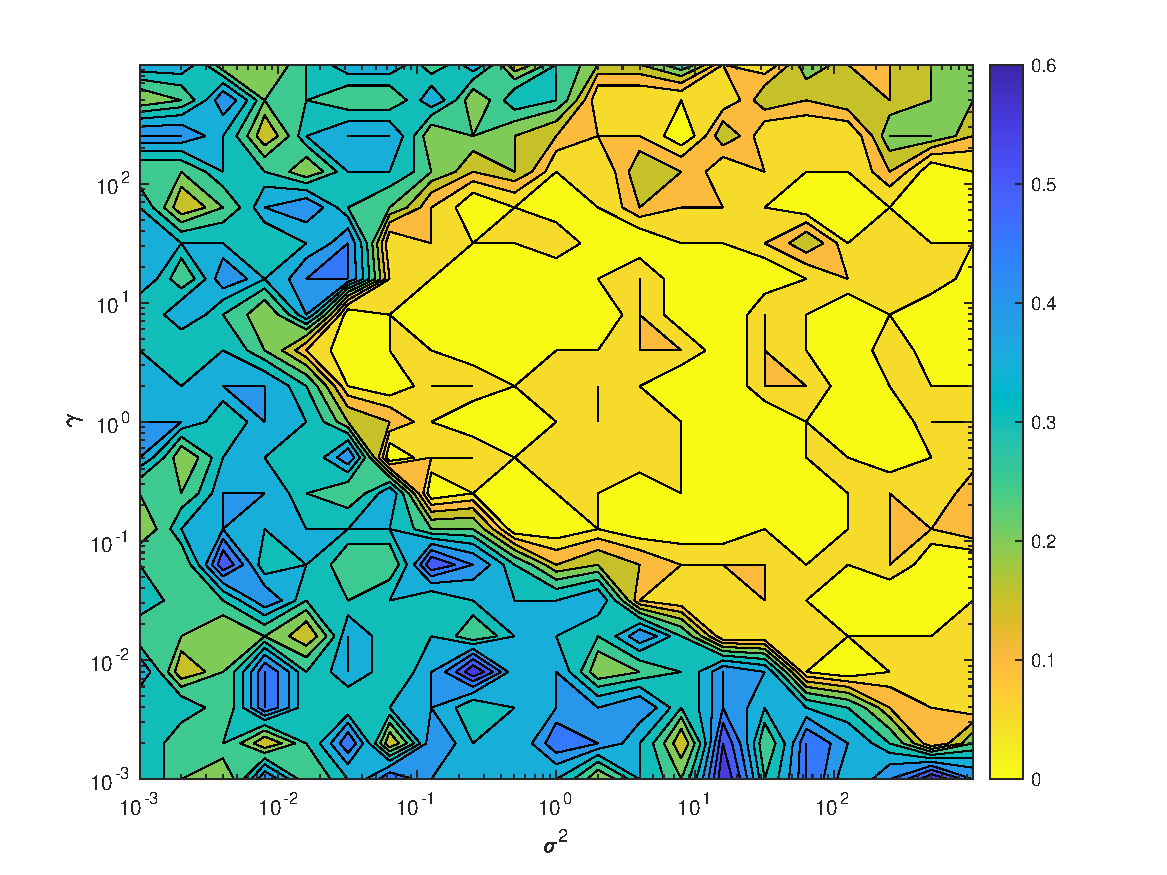
\includegraphics[width=0.33\textwidth]{../src/figures/iris/validation_2}}\hfil
\subfloat[Leave-one-out validation.]{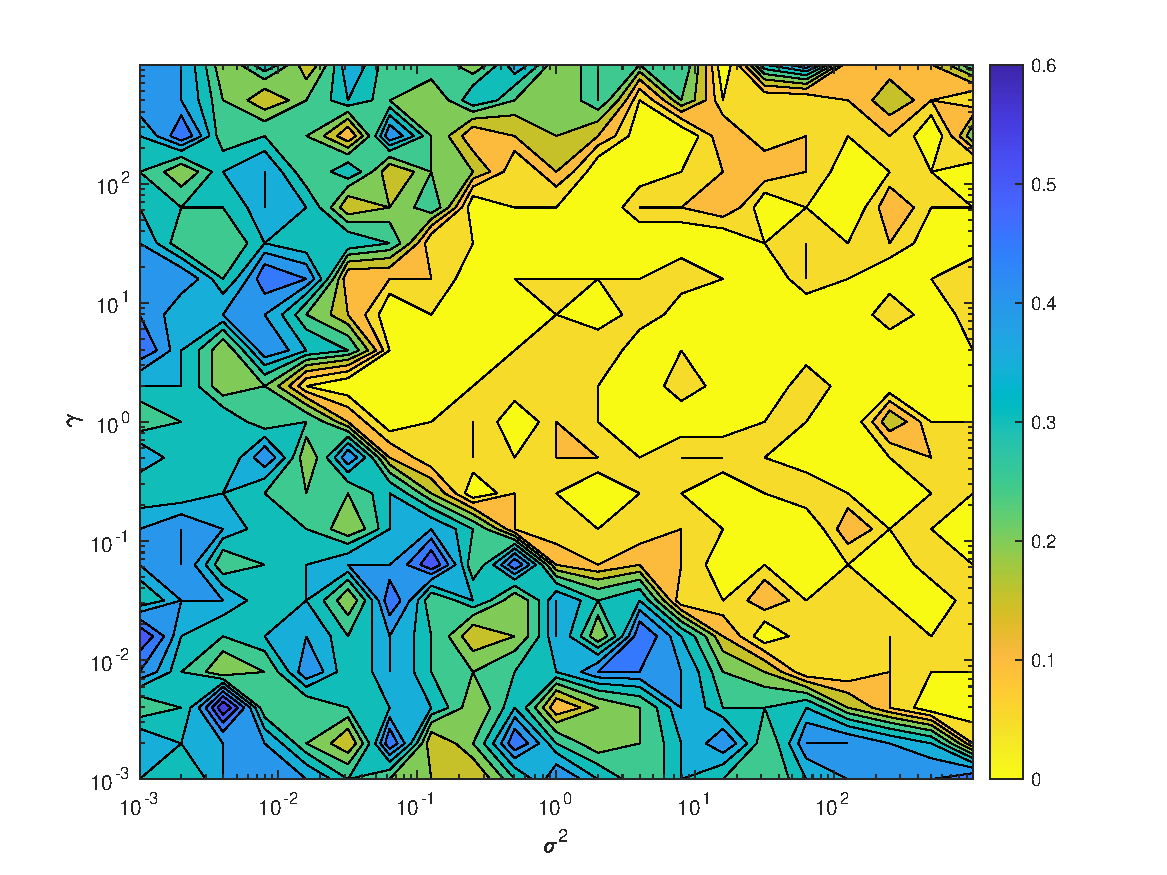
\includegraphics[width=0.33\textwidth]{../src/figures/iris/validation_3}}\hfil
\caption{Grid search in conjunction with various validation techniques. The results differ and the results for the random split strategy varies between runs. $k$-fold crossvalidation appears to be a better approximation of the error but may generalise less well. Reasonable parameters lie in the yellow zone where the error reaches a maximum of about 10\%. A small bandwidth of between say, 0.1 and 1.0 and a regularization constant of 1.0 seems reasonable.}
\label{validation}
\end{figure}

\begingroup
\setlength{\columnsep}{0.75cm}
\setlength{\intextsep}{0.2cm}
\begin{wrapfigure}{l}{0pt}
	\centering
       	 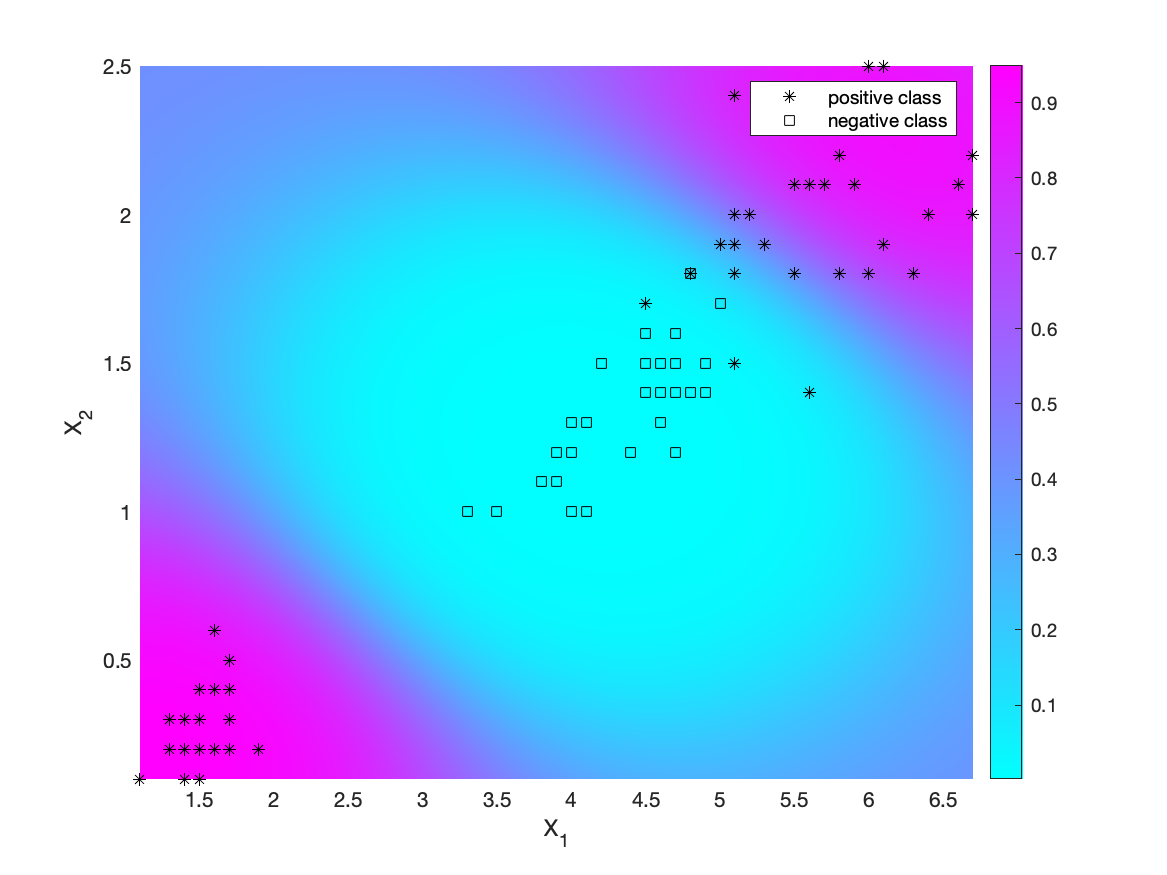
\includegraphics[width=0.45\textwidth]{../src/figures/iris/bayesian/bayesian_probabilities}
        	\caption{Posterior probability estimates using a Bayesian approach ($\gamma\approx0.038,\sigma^2\approx 0.56$). The hue indicates the probability that the data point at a location in the 2-dimensional plane belongs to one or the other class. A smaller $\sigma^2$ can lead to overfitting and makes for a more clearly defined, smaller blue area.}
	\label{irisbayesian}
\end{wrapfigure}

An ROC curve can be generated for any model. One calculates the result of the model applied on every test data point and uses the results as thresholds for which the true positive rate (TPR) is plotted in function of the false positive rate (FPR). The area under the curve (AUC) can then be used to gauge the effectiveness of the classifier. For $\gamma=0.037622,\sigma^2=0.559597$ it happens to equal 1 indicating a perfect classifier. If the \texttt{sign} function had been used to classify test data there would be a misclassification error (the FPR would be 0.1).

\par Using a Bayesian approach (considered in greater detail in the second part of this report) which requires a prior denoting the probability of occurrence of each class it is possible (by applying Bayes' theorem) to estimate the probability that a given data point belongs to the positive or the negative class. A corresponding plot of these posterior probabilities for the same model used to calculate the ROC curve is shown in figure \ref{irisbayesian}. The prior is taken to be 0.67 (the classes are unbalanced).

\endgroup

%
%\begin{figure}[htp]
%\centering
%\subfloat[Ripley dataset.]{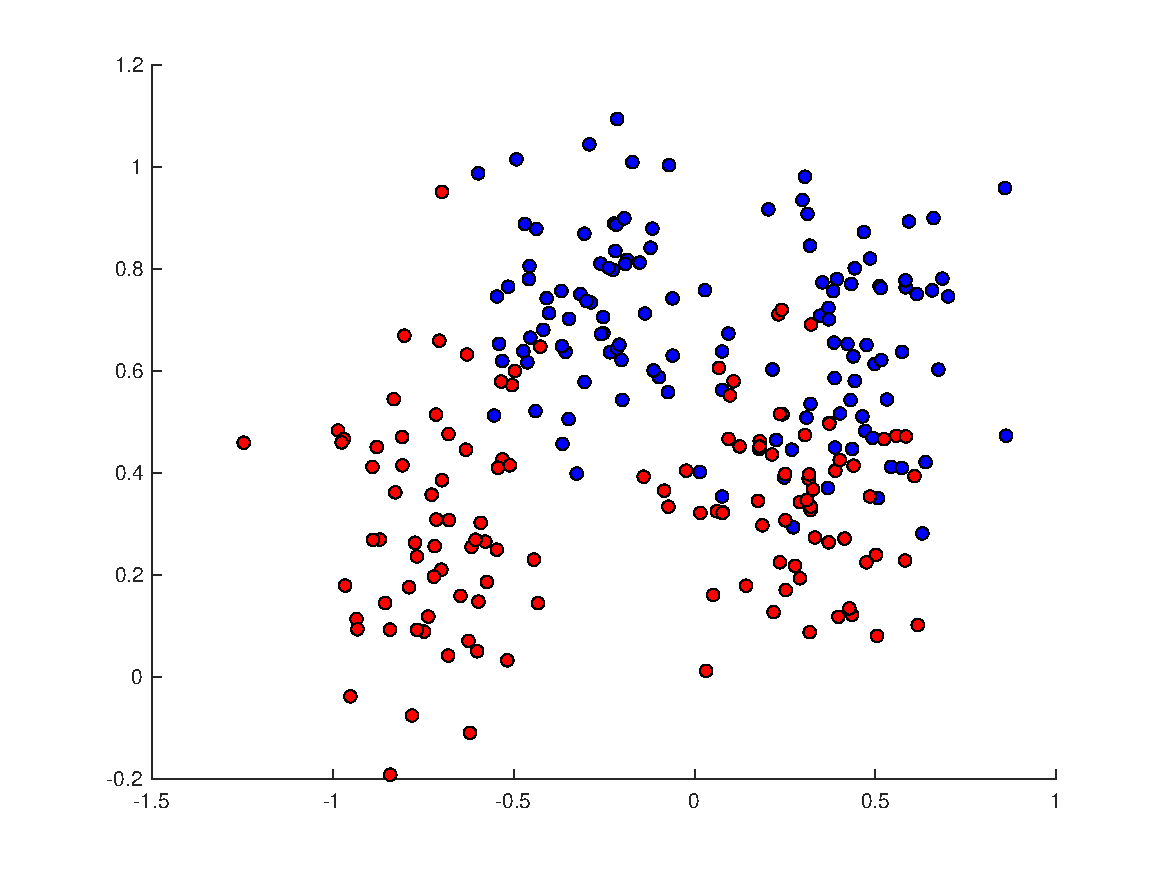
\includegraphics[width=0.33\textwidth]{../src/figures/classification/ripley}}\hfil
%\subfloat[Wisconsin breast cancer dataset.]{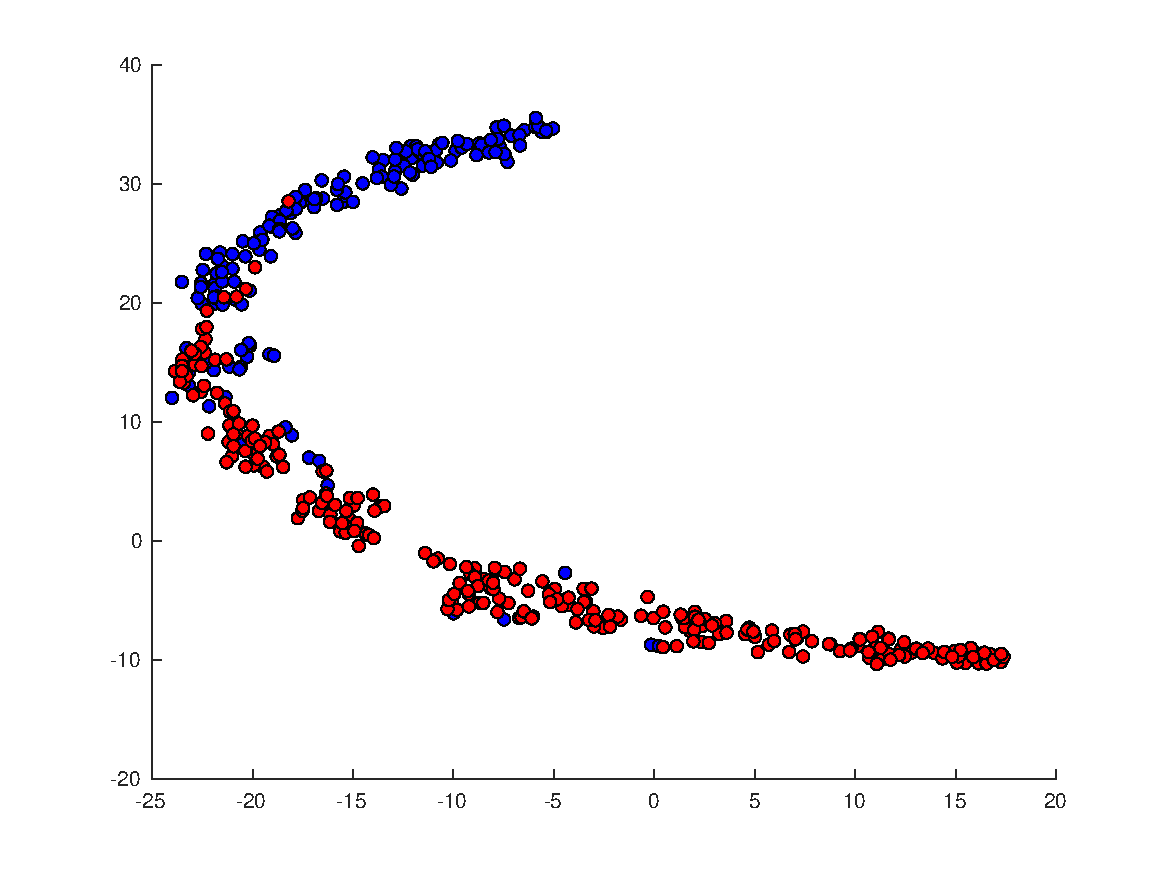
\includegraphics[width=0.33\textwidth]{../src/figures/classification/wisconsin}}\hfil
%\subfloat[Diabetes dataset.]{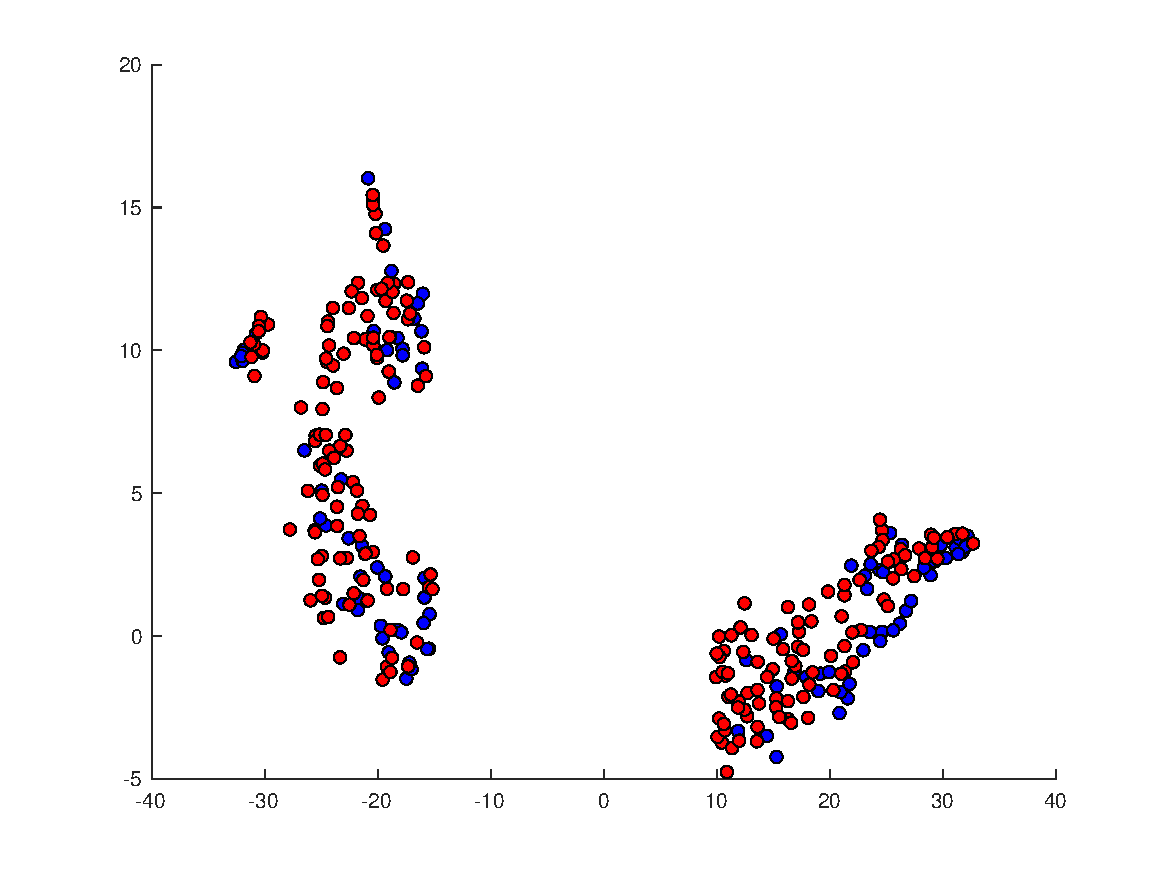
\includegraphics[width=0.33\textwidth]{../src/figures/classification/diabetes}}\hfil
%\caption{Visualisation of three datasets : the Ripley, Wisconsin breast cancer - and diabetes dataset.}
%\label{datasets_vis}
%\end{figure}

\fakesubsection{Ripley dataset}{}

\begin{figure}[htp]
\centering
\subfloat[Ripley dataset.]{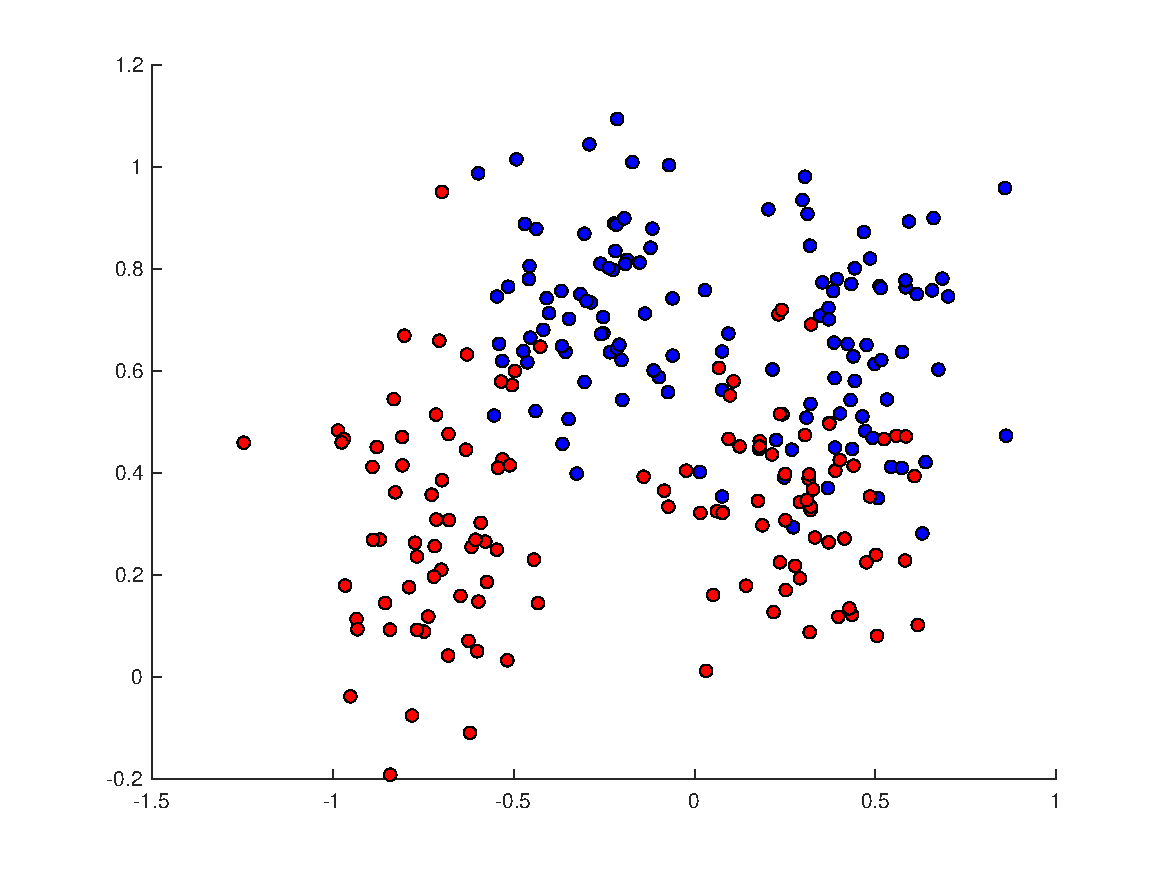
\includegraphics[width=0.32\textwidth]{../src/figures/classification/ripley}}\hfil
\subfloat[Results with a linear kernel (tuned parameter $\gamma\approx 0.0027$, misclassification rate of $10.2\%$, AUC $\approx 0.956$).]{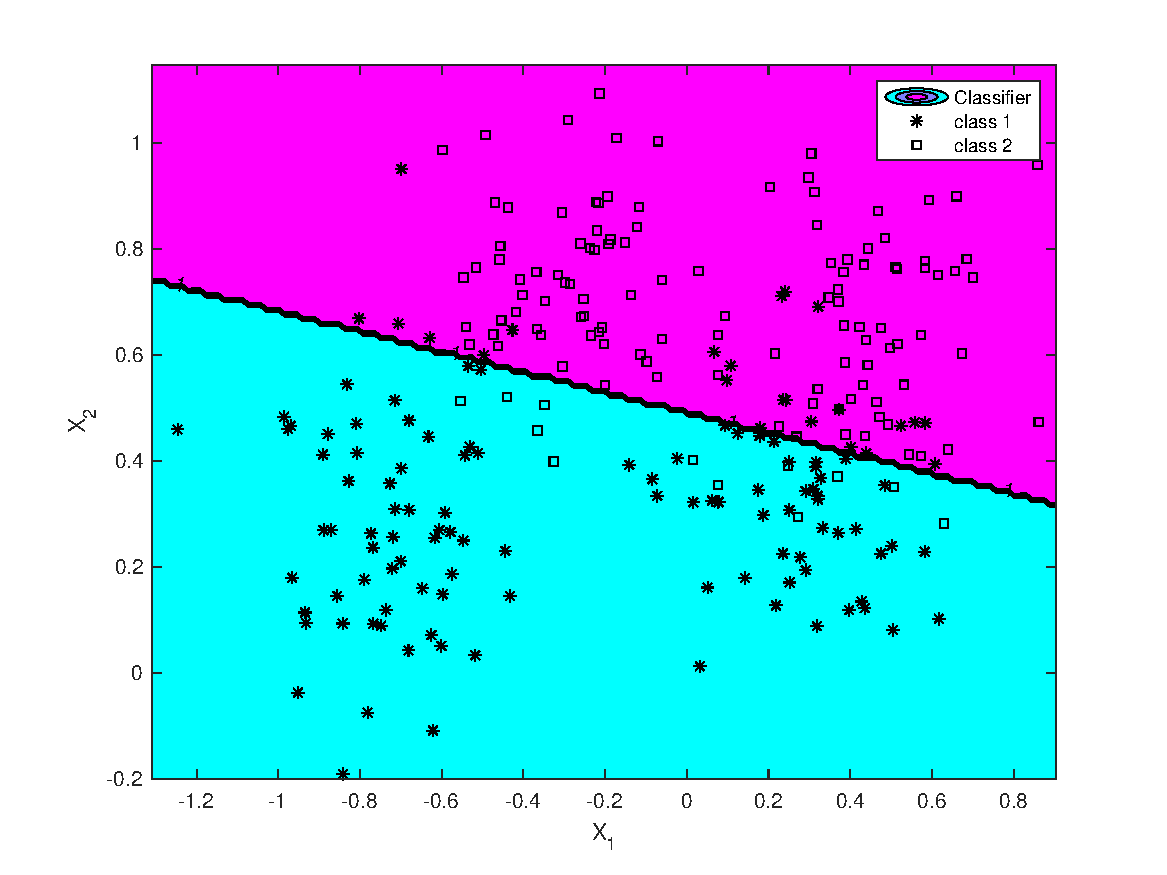
\includegraphics[width=0.32\textwidth]{../src/figures/classification/ripley_lin_kernel}}\hfil
\subfloat[Results with an RBF kernel (tuned parameters $\gamma\approx 0.537,\sigma^2\approx 0.338$, misclassification rate of $9.1\%$, AUC $\approx 0.968$).]{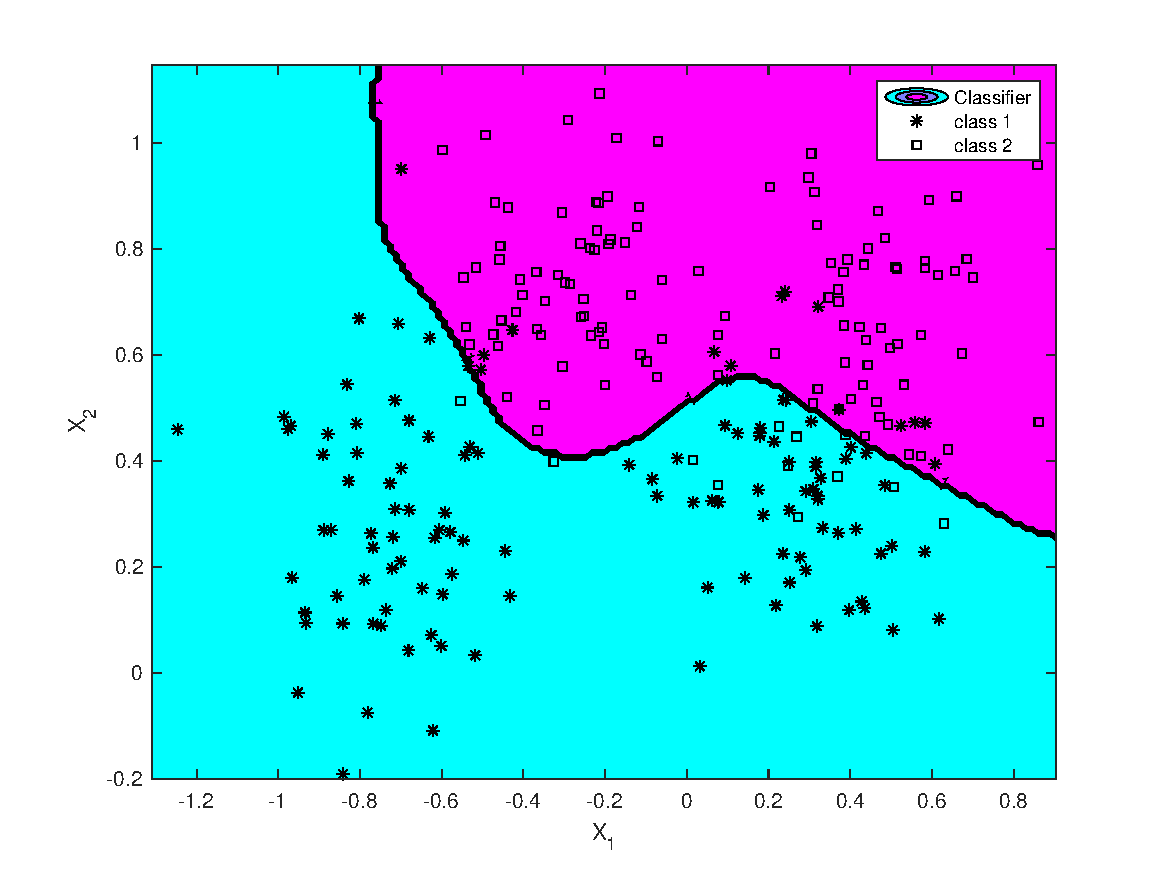
\includegraphics[width=0.32\textwidth]{../src/figures/classification/ripley_RBF_kernel}}\hfil
\caption{The Ripley dataset and results with a linear and an RBF kernel. LSSVMs are used. The number of support vectors equals 250 (100\%) in all cases.}
\label{ripley}
\end{figure}

The Ripley dataset is a 2-dimensional so it can easily be visualised (figure \ref{ripley}). The data for each class is generated by a mixture of two Gaussian distributions and it is not linearly separable in the input space. The distributions were chosen as to \textit{`allow a best-possible error rate of about 8\%'}, each component has the same covariance matrix (basically a 2-component version of the introductory example). The data is a \textit{`realistic'} toy problem and it is rather noisy.

\par An LS-SVM with a linear kernel makes for a classification rate of around 10\% while an RBF kernel performs a tad better at a rate of about 9\% (and so does a polynomial one\footnote{Automated tuning of the polynomial usually resulted in a degree $\delta$ between 4 and 7.}). The ROC curves give a more complete picture and aren't shown here, but the AUC was the highest for the RBF kernel (about 0.97) with accuracy being the highest at a threshold a bit below zero. In practice (when met with real-life datasets) other operating points may be chosen depending on the cost of each type of misclassification.

\par Steve Gunn's \texttt{MATLAB} toolbox which is also used for regression in the second part of the report provides functions for generating classical SVMs and some more kernels that can be experimented with though it provides no automated tuning method for these. The results for linear -, RBF and polynomial kernels are about the same though there are less support vectors. Results after manual tuning (through the \texttt{uiclass} interface) are shown in figure \ref{ripleysvm}.

\begin{figure}[htp]
\centering
\subfloat[Linear kernel ($\gamma=1.0,\rho=11.5\%$, 125 support vectors)).]{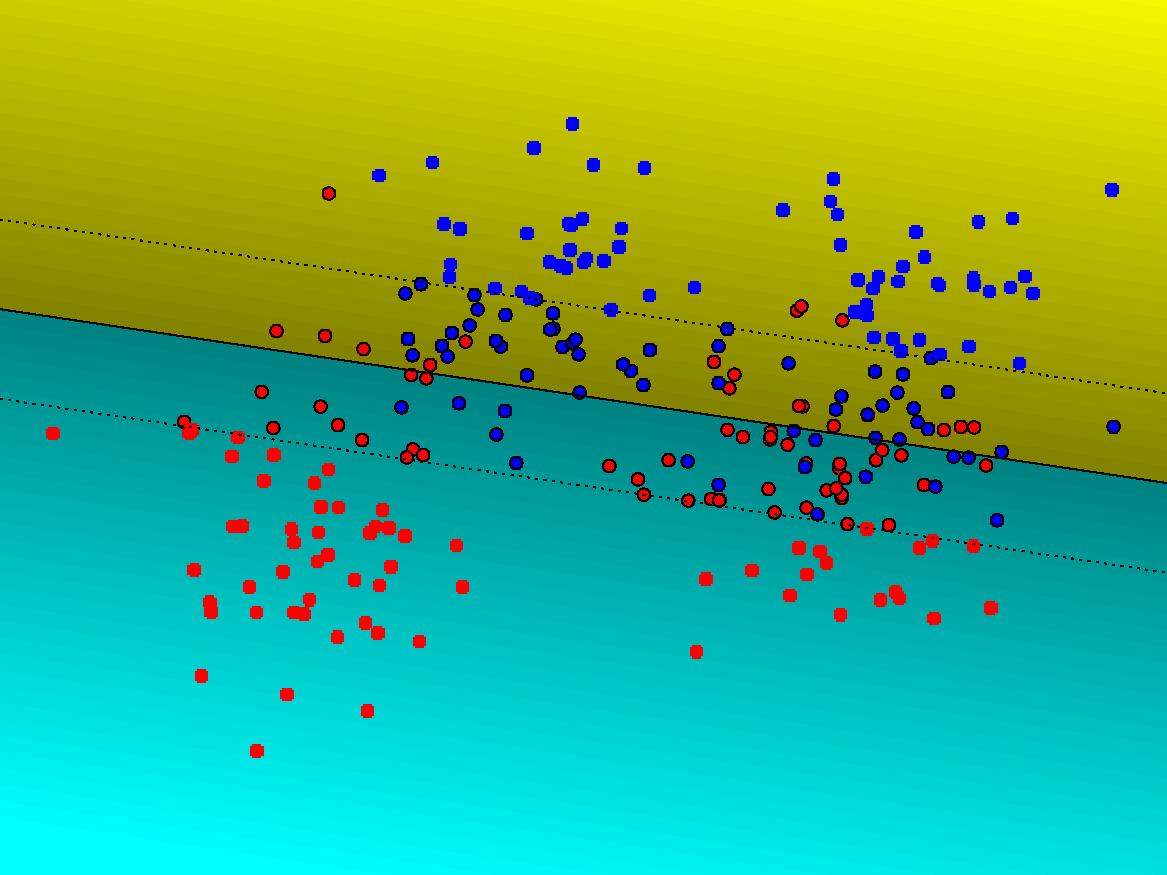
\includegraphics[width=0.28\textwidth]{../src/figures/classification/ripley_svm_linear}}\hfil
\subfloat[Polynomial kernel ($\delta=5,\gamma=1.0,\rho=10.0\%$, 77 support vectors)).]{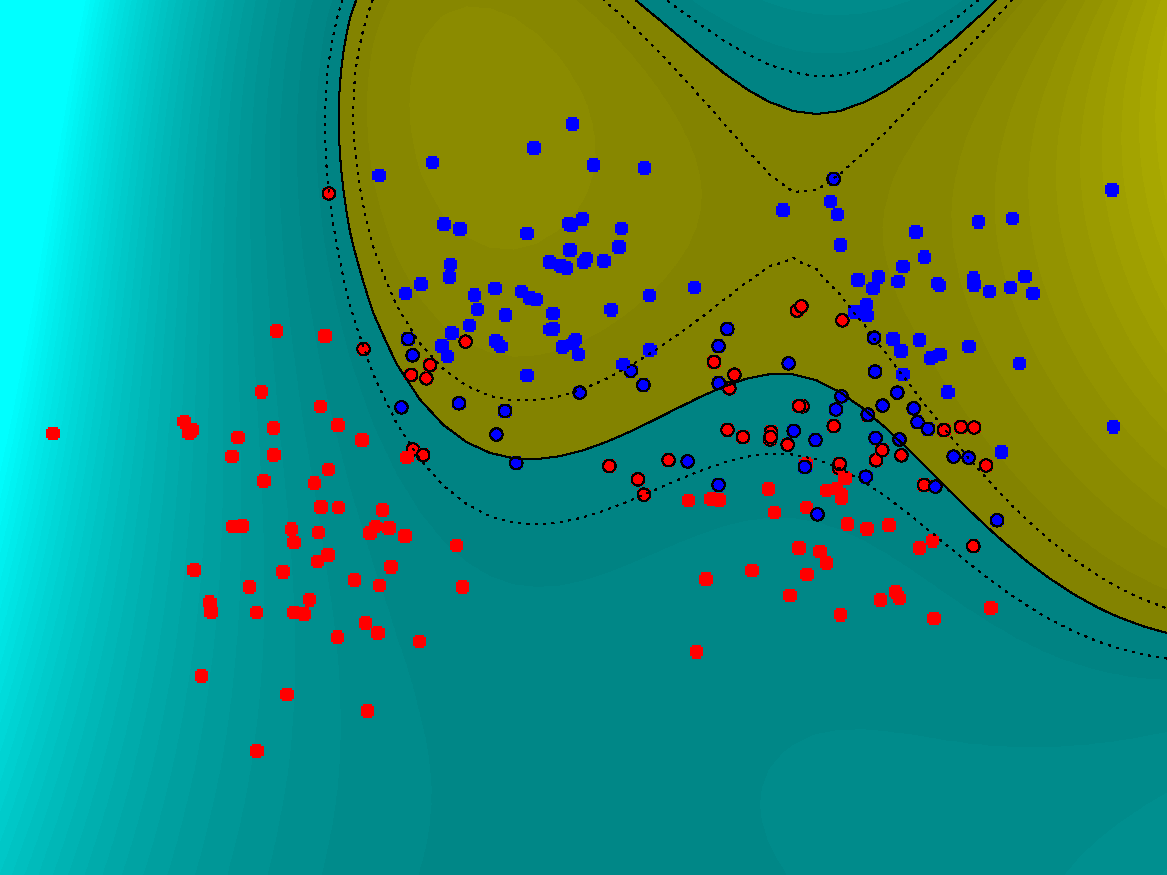
\includegraphics[width=0.28\textwidth]{../src/figures/classification/ripley_svm_poly}}\hfil
\subfloat[RBF kernel ($\gamma=0.5,\sigma^2=0.15,\rho=9.2\%$, 124 support vectors).]{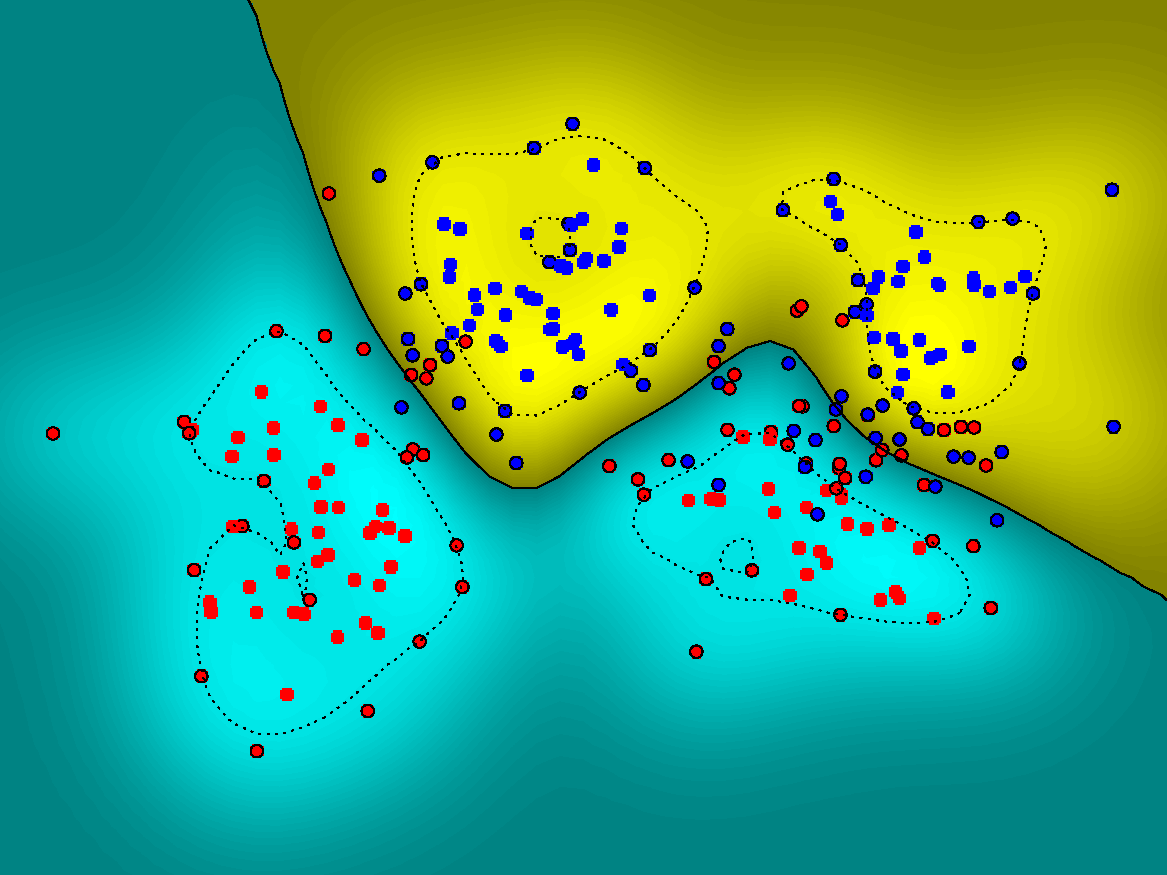
\includegraphics[width=0.28\textwidth]{../src/figures/classification/ripley_svm_rbf}}\hfil
\caption{The Ripley dataset and results with a linear and an RBF kernel. LSSVMs are used.}
\label{ripleysvm}
\end{figure}

Since the dataset is Gaussian an RBF kernel should be an appropriate pick. As it's also a noisy dataset a smoother decision surface (higher $\sigma^2$ and/or lower $\gamma$) should be opted for. Of course in this case the optimal classifier (in terms of maximisation of the posterior probabilities) can be defined based on Bayes' theorem.

\fakesubsection{Wisconsin breast cancer dataset}{}

With 30 features for each of the observations the Wisconsin breast cancer diagnosis dataset isn't trivial to visualise. \texttt{MATLAB} has an implementation of t-SNE or two principal components determined through PCA could be plotted. Distributions of some of the features are shown below. The two classes denote benign - or malignant cancer tissue. In contrast with the previous dataset this one's a bit unbalanced ($62.5\%$ belongs to the negative class) which can be accounted for through bias correction\footnote{Whilst doing so it came to my attention that the \texttt{roc} function in the LS-SVM toolbox \textit{seems} to return the thresholds in the wrong (reverse) order.} or by using weights in the SVM formulation to give more emphasis to the terms associated to the minority class. 

\vspace{-0.5cm}
\begin{figure}[htp]
\centering
\subfloat[Mean radius.]{\includegraphics[width=0.25\textwidth]{../src/figures/classification/breast_hist_1}}\hfil
\subfloat[Mean texture.]{\includegraphics[width=0.25\textwidth]{../src/figures/classification/breast_hist_2}}\hfil
\subfloat[Mean perimeter.]{\includegraphics[width=0.25\textwidth]{../src/figures/classification/breast_hist_3}}\hfil
\subfloat[Mean area.]{\includegraphics[width=0.25\textwidth]{../src/figures/classification/breast_hist_4}}\hfil
\caption{Distributions of the first 4 features of the Wisconsin breast cancer dataset (red denotes malignant -, blue denotes benign tumors). There are 10 features in total and for each of these the mean, standard error and maximum value is given. For some of the features none of those three appear to be particularly informative.}
\label{breasthist}
\end{figure}

\par A simple automated tuning experiment of an LS-SVM with linear -, polynomial - and RBF kernels yielded average AUCs of $0.996\pm 0.001$, $0.937\pm 0.058$ and $0.995\pm 0.002$ respectively. It may be surprising that a linear kernel outperformed a non-linear one - the number of features is larger and there's not that many data points so a simpler decision boundary may help to avoid overfitting since Cover's theorem implies that it is more likely that the data is linearly separable when the number of dimensions is high (and the number of data points is low).

\par As some of the features seem less informative than others it may be worthwhile to remove some of them either through PCA or a more sophisticated approach like automatic relevance determination. A basic experiment ended up with the latter selecting 21 features. Training the model on these resulted in an AUC of 0.9973. The results with a larger number of tuning and training runs as well as a comparison with a basic PCA approach are shown in table \ref{breasttab}.

\begin{table}
\centering
\begin{tabular}{c|ccccc}
& ARD (RBF kernel) & PCA ($n_h=2$) & PCA ($n_h=3$) & PCA ($n_h=10$)\\\hline
Cost & $2.075\% \pm 0.206$ & $6.125\% \pm 0.339$ & $3.825\% \pm 0.237$ & $3.750\% \pm 0.167$\\
AUC & $0.99723 \pm 0.00040$ & $0.98402 \pm 0.00335$ & $0.99077 \pm 0.00238$ & $0.98729 \pm 0.00520$
\end{tabular}
\caption{Mean and standard deviation of accuracy and AUC for linear kernel models after application of two types of dimensionality reduction ; PCA or automatic relevance determination (which selected 21 features). PCA was applied by subtracting the mean, applying PCA on the training set and using the resulting projection on both the training - and test set after which an LS-SVM with an RBF kernel was tuned and trained. A linear kernel wasn't as performant as the number of dimensions decreased.}
\label{breasttab}
\end{table}

\fakesubsection{Diabetes dataset}{}

% and an overview of the 3 new kernels that were tried are given here :
%
%\begin{table}[h]
%\centering
%\begin{tabular}{c|cp{0.65\textwidth}}
%\textit{Kernel} & \textit{Parameters} & \textit{Description} \\\hline
%\textit{Sigmoid} & $\alpha$ (scale) and $c$ (offset) & A multilayer perceptron kernel $k(x,y)=tanh(\alpha\cdot x^T\cdot y+c)$ equivalent to using a 2-layer perceptron. \\
%\textit{Spline} & parameter & aaa \\
%\textit{B-spline} & parameter & aaa \\
%\end{tabular}
%\label{misckernels}
%\caption{Miscellaneous kernels experimented with for the Ripley dataset.}
%\end{table}

